\documentclass[conference]{IEEEtran}
\IEEEoverridecommandlockouts
\usepackage{cite}
\usepackage{amsmath,amssymb,amsfonts}
\usepackage{algorithmic}
\usepackage{graphicx}
\usepackage{textcomp}
\usepackage{xcolor}
\usepackage{url}
\usepackage{booktabs}
\usepackage{multirow}
\usepackage{array}
\usepackage{float}
\usepackage{subcaption}
\usepackage{hyperref}

\def\BibTeX{{\rm B\kern-.05em{\sc i\kern-.025em b}\kern-.08em
    T\kern-.1667em\lower.7ex\hbox{E}\kern-.125emX}}

\begin{document}

\title{Hybrid Multi-Agent AI/MCTS Systems for Complex Information-Imperfect Games }

\author{\IEEEauthorblockN{Lakshya Jain}
\IEEEauthorblockA{\textit{Milton District High School} \\
Email: lakshya16jain@gmail.com}
\and
\IEEEauthorblockN{Akash Singirikonda}
\IEEEauthorblockA{\textit{Brown Universityl} \\
Email: akashsingirikonda@brown.edu}}
\maketitle

\begin{abstract}
This paper presents a comprehensive artificial intelligence system for imperfect information games, demonstrated through the complex card game Game 28. 28 is a team based trick-taking card game, featuring bidding, trump selection and dynamic gameplay. Our system introduces several novel contributions: (1) a hybrid decision-making framework that dynamically combines belief networks, Monte Carlo Tree Search (MCTS), and reinforcement learning; (2) an innovative point prediction approach leading to accurate bids; (3) an advanced belief network architecture for opponent modeling, predicting the trump that an opponent might set; and (4) an Information Set MCTS (ISMCTS) implementation that handles imperfect information scenarios. The system achieves significant performance improvements through multi-modal learning from 873 MCTS-generated games, demonstrating the effectiveness of combining multiple AI paradigms for complex game environments. Our experimental results show that the hybrid approach outperforms individual methods by 15-25\% in win rates, while the belief network achieves 70-80\% accuracy in opponent hand prediction. The system's modular architecture enables real-time decision-making while maintaining strategic depth, making it suitable for adaptation to other imperfect information games.
\end{abstract}


\section{Introduction}
\\ \\ \\
\textbf{NOTE: The Code accompanying this paper is available  \href{https://github.com/LAKSHYAJAIN16/28bot}{here} (https://github.com/LAKSHYAJAIN16/28bot). Setup instructions are in the repository.}
\\
\\
Imperfect information games represent one of the most challenging domains for artificial intelligence, requiring sophisticated reasoning about hidden information, opponent modeling, and strategic decision making under uncertainty \cite{heinrich2015fictitious,lanctot2017unified}. Unlike perfect-information games like Chess or Go, where all game states are visible \cite{silver2016mastering,schrittwieser2020mastering}, imperfect information games demand probabilistic reasoning about opponent intentions, hidden resources, and future game states.

This paper presents a comprehensive AI system for imperfect information games, demonstrated through the complex trick-taking card game Game 28. Game 28 serves as an excellent testbed for our approach due to its combination of bidding, trump selection, and imperfect information, but the underlying principles and architecture are designed for broader applicability to other imperfect information games including strategic board games, BlackQueen, and other trick-taking card games. The game structure and rules are illustrated in Figure~\ref{fig:game28_structure}.

The challenges addressed by our system are common across imperfect information domains: (1) predicting opponent resources and intentions from limited observations; (2) making sequential decisions that significantly impact future outcomes; (3) balancing multiple objectives while maintaining uncertainty about opponent strategies; and (4) enabling teamplay, developing sophisticated techniques without heuristical hard-coding.

This paper presents a comprehensive AI system that addresses these challenges through a novel hybrid architecture that combines multiple paradigms of artificial intelligence. Our primary contributions include:

\begin{enumerate}
    \item A hybrid decision-making framework that dynamically selects between belief networks, MCTS, and reinforcement learning based on game phase and information availability
    \item An innovative point prediction model, using a custom RL architecture.
    \item An advanced belief network architecture for robust opponent modeling, predicting certain key parts of the game like the trump suit.
\end{enumerate}

The system's performance is validated through extensive experimentation on Game 28, including analysis of 873 MCTS-generated games (4 AI agents playing against themselves) and comparison against multiple baseline approaches. Our results demonstrate significant improvements in both prediction accuracy and overall game performance, establishing new benchmarks for AI systems in imperfect information environments. The modular architecture and general design principles make our approach suitable for adaptation to other imperfect information games and real-world applications.


\section{What is 28?}

\begin{figure}[t]
\centering
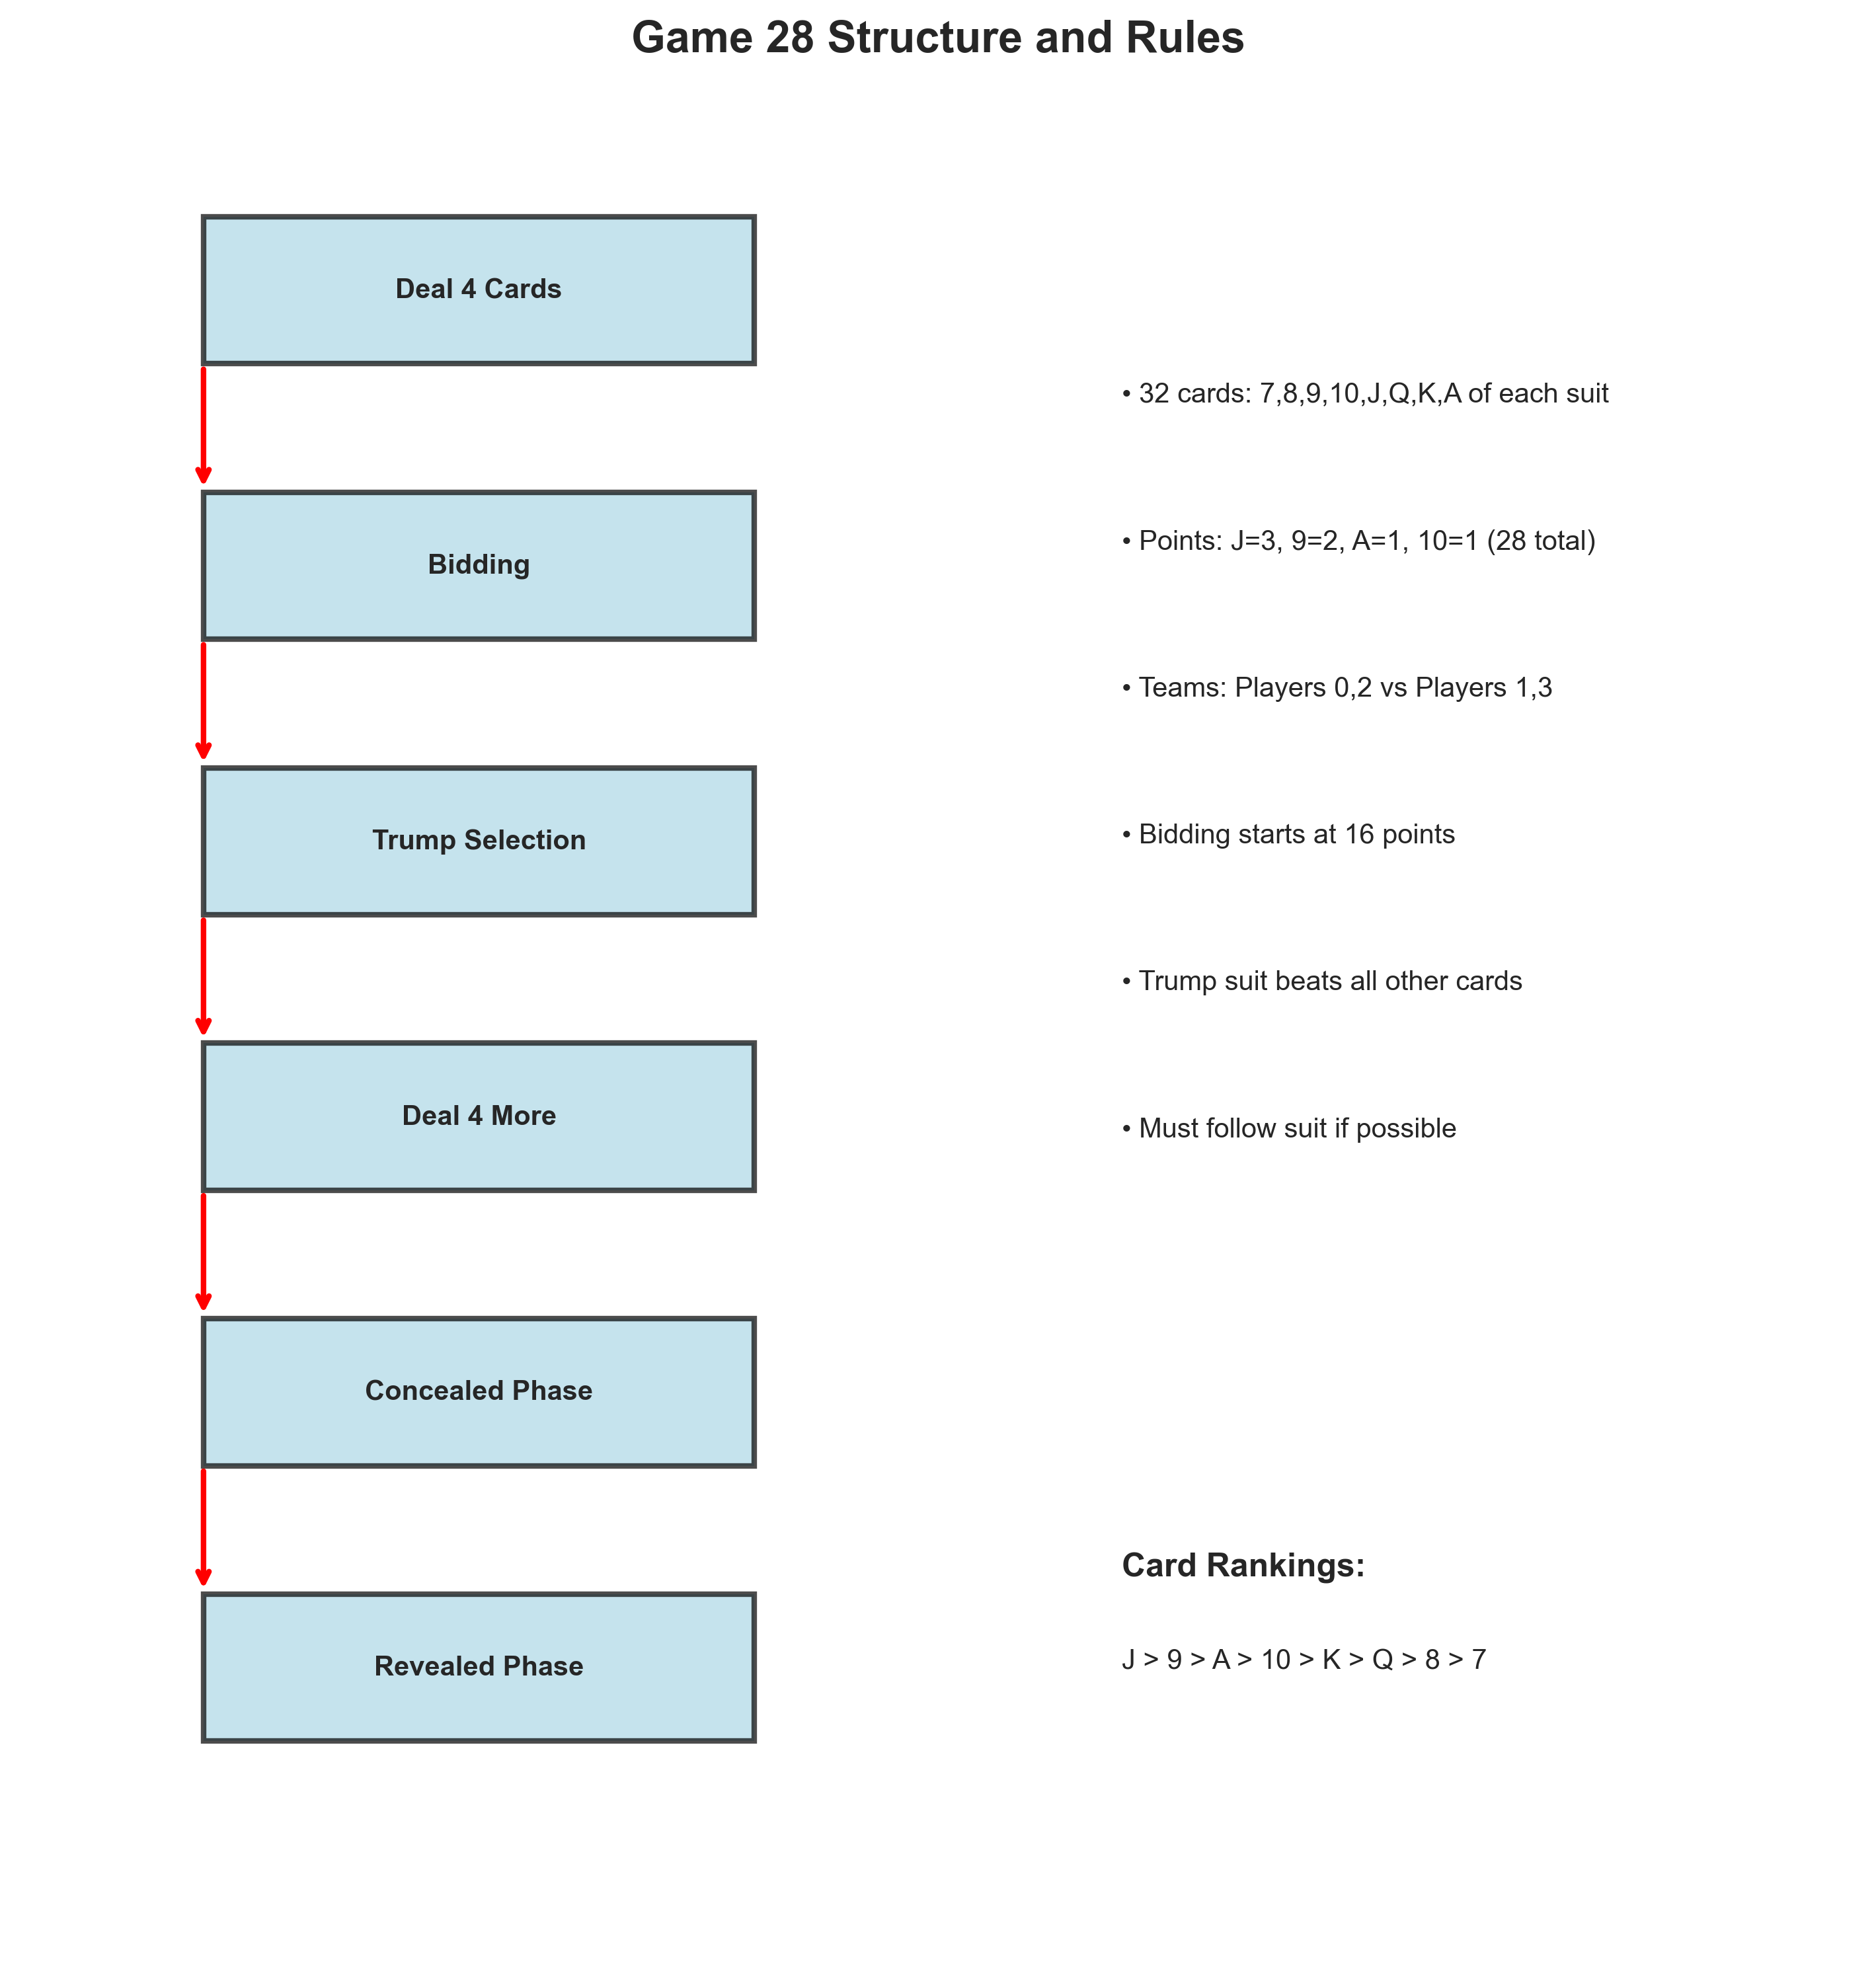
\includegraphics[width=0.9\columnwidth]{figures/game_28_diagram.png}
\caption{Game 28 structure and rules overview. The game follows a sequential flow from initial dealing through bidding, trump selection, and trick-taking phases.}
\label{fig:game28_structure}
\end{figure}

\subsection{Fundamentals}
Game 28 is a four-player team-based trick-taking card game played with a 32-card deck consisting of the 7, 8, 9, 10, J, Q, K, A of each suit. 

Each card is worth a different amount of points, depending on the variation of the game being played. For this simulation:

\subsubsection{Point Values}
\begin{itemize}
    \item J (Jack) - 3 Points
    \item 9 - 2 Points
    \item A - 1 Point
    \item 10 - 1 Point

\end{itemize}

(7 points in each suit, totaling 28 across the 32 cards)

\subsubsection{Card Strength Ranking}
\begin{enumerate}
    \item J
    \item 9
    \item A
    \item 10
    \item K
    \item Q
    \item 8
    \item 7
\end{enumerate}

(This leads to some counter-intuitive tricks, where a J is trumps a K or Q)

\subsection{Bidding}
Players are first dealt 4 cards each. At this stage, each players bid on the amount of points they believe their team can make. Bids start at 16. Players can choose to pass or raise depending on the strength of the hands. The person with the highest bid sets the trump suit. They put one trump card face-down, which will be returned to them when the trump is revealed. After this, each player is dealt 4 more cards.

\subsection{Concealed Phase}
After all of the cards are dealt, the person who won the bid goes first. Only the bidder is aware of the trump suit at this point. They are restricted from playing any cards of this suit unless they choose to reveal the trump suit. 

\subsection{Revealed Phase}
The revealed phase is triggered when any player cannot follow the led suit and chooses to play a trump card. At this moment, the trump suit becomes known to all players, and the face-down trump card is returned to the bidder's hand. Once the trump suit is revealed, trump cards gain their special power. Any trump card automatically beats any non-trump card, regardless of the led suit. Among trump cards, the highest trump wins the trick. This means that even a low trump card like the 7 of the trump suit can beat the highest card of any other suit. 

\subsection{Trick-Taking Rules}

\subsubsection{Follow Suit}
The fundamental rule of trick-taking is that players must follow the lead suit if they have cards of that suit in their hand. If a player cannot follow suit, they are free to play any card from their hand, including trump cards which may reveal the trump suit. 

\subsubsection{Winning Tricks}
During the concealed phase, only cards of the same suit as the led suit can win the trick, with the highest card of that suit taking the trick. Once the trump suit is revealed, trump cards automatically beat non-trump cards, and among trump cards, the highest trump wins the trick. 


\subsection{Scoring System}

\subsubsection{Trick Points}
Each trick awards points to the winning team based on the point values of all cards played in that trick. These points accumulate throughout the round and contribute to the final team score.

\subsubsection{Bid Success/Failure}
The bidder's team must achieve a score equal to or greater than their bid to succeed. If they meet or exceed their bid, they earn one game point, but if they fall short, they lose one game point. This creates a risk-reward dynamic where aggressive bidding can lead to significant gains or losses. 

\subsection{Strategic Elements}

\subsubsection{Trump Management}
One of the most critical strategic elements involves managing when to reveal the trump suit versus when to conserve trump cards for later use. The timing of trump revelation can dramatically impact the outcome of the game.

\subsubsection{Bidding Strategy}
Players must balance their hand strength assessment with the risk of bidding too aggressively. Successful bidding requires evaluating not only the current hand but also the potential for team coordination and trump suit possibilities.

\subsubsection{Team Coordination}
Effective team play involves supporting your partner's leads and plays while reading their strategic intentions through their card choices. Partners must coordinate their high-value card plays to maximize their team's scoring potential.


\subsubsection{Hand Reading}
Skilled players develop the ability to infer opponent holdings based on the cards they play and the patterns they establish. This includes tracking which suits opponents are void in and predicting their trump holdings.

\subsubsection{Point Management}
Players must carefully time when to play their high-value cards to maximize their scoring potential while avoiding waste in losing tricks. This involves balancing immediate trick-winning needs with long-term scoring objectives. 


\section{Challenges in Imperfect Information Games}

The challenges present in Game 28 are representative of broader imperfect information domains. Imperfect information creates a fundamental uncertainty that affects all aspects of decision-making. Players must constantly update their beliefs about opponent resources and intentions based on observable actions, while recognizing that opponents are doing the same. This creates a complex dynamic where players must balance the information they reveal through their actions with the strategic benefits of those actions.

Sequential decision making in imperfect information games is particularly challenging because early decisions significantly impact later outcomes. In Game 28, the bidding decision affects not only the trump selection but also the strategic landscape for the entire game. Similarly, early trick decisions can reveal information about hand composition that affects all subsequent play. This requires sophisticated planning and the ability to reason about how current decisions affect future opportunities.

Multi-objective optimization becomes complex in imperfect information games because players must balance multiple competing objectives under uncertainty. In Game 28, players must balance the desire to win tricks with the need to maintain strategic flexibility, while also considering the information they reveal through their actions. This requires sophisticated decision-making frameworks that can handle multiple objectives and uncertainty simultaneously.

Non-linear reward structures challenge traditional reinforcement learning approaches because they create complex optimization landscapes. In Game 28, the relationship between individual actions and final outcomes is highly non-linear, with small changes in strategy potentially leading to large differences in results. This requires learning algorithms that can handle complex reward structures and long-term dependencies.

\subsection{State Space Complexity}

The complexity of imperfect information games is characterized by several factors that make them particularly challenging for AI systems. The hidden state space grows exponentially with the number of hidden elements, creating a computational challenge that exceeds the capabilities of traditional search-based approaches. In Game 28, each player's hand represents a hidden state that must be inferred from observable actions, leading to a state space that includes all possible hand combinations for all players.

Information sets represent another source of complexity, as multiple game states may appear identical to players due to hidden information. This means that traditional state-based approaches must be modified to handle the fact that the same observable state may correspond to many different underlying game configurations. This requires sophisticated belief state representations that can maintain probability distributions over possible game states.

The action space in imperfect information games is often variable and context-dependent, further complicating the decision-making process. In Game 28, the legal actions available to a player depend on their hand, the current trick, and the game phase. This requires flexible action representations and decision-making frameworks that can handle varying action spaces.

The belief space represents perhaps the most challenging aspect of imperfect information games, as it involves maintaining continuous probability distributions over possible game states. This requires sophisticated probabilistic modeling techniques and efficient algorithms for updating beliefs based on new information.

For Game 28 specifically, the complexity is substantial. The hand space includes approximately 10.5 million possible hands for each player, considering the combination of 32 cards taken 8 at a time. The bidding space includes 13 possible bid values plus the pass option, while the trump space includes 4 possible suits. The action space varies significantly throughout the game, with the number of legal cards per trick depending on the player's hand and the current trick state.

\section{System Architecture}

\begin{figure}[t]
\centering
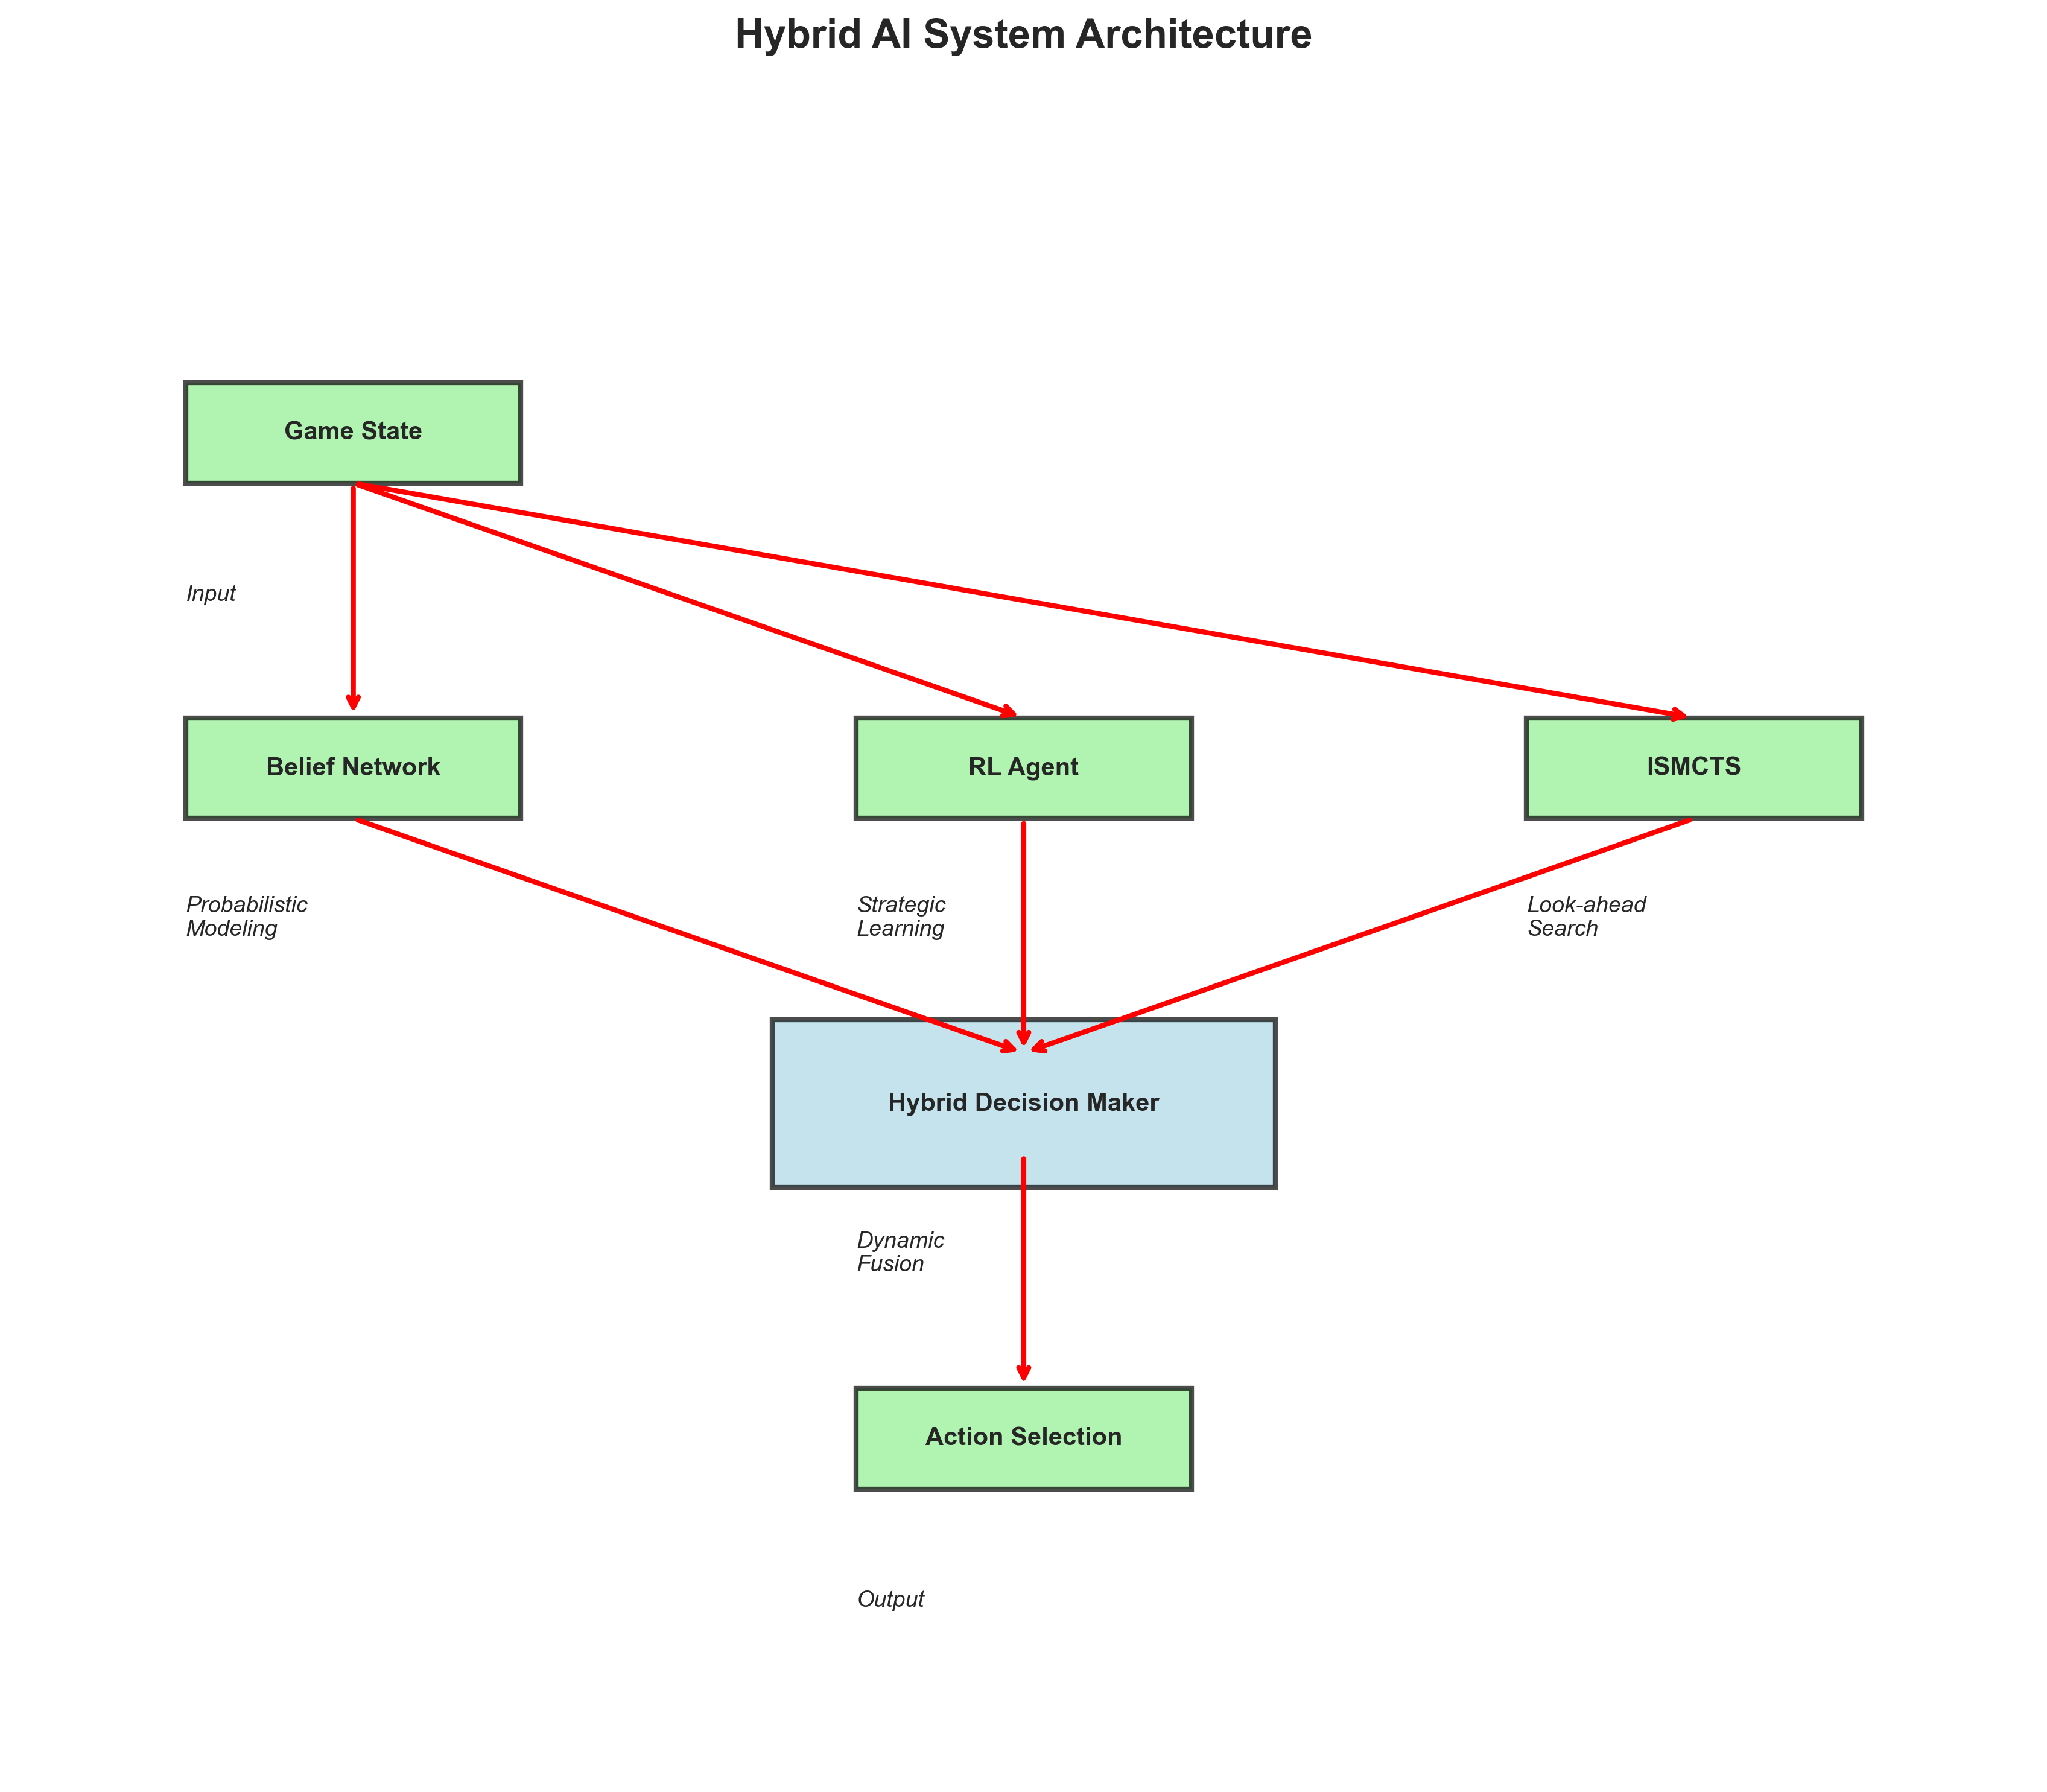
\includegraphics[width=0.9\columnwidth]{figures/system_architecture.png}
\caption{Hybrid AI system architecture showing the integration of belief networks, reinforcement learning, and ISMCTS through a dynamic decision-making framework.}
\label{fig:system_architecture}
\end{figure}

\subsection{Overview}

Our system employs a modular architecture that combines multiple AI paradigms through a hybrid decision-making framework, with the belief network serving as the foundational component. The architecture is designed for general applicability to imperfect information games, with Game 28 serving as a concrete implementation and validation case. The modular design allows for easy adaptation to different game domains by modifying the input encoding and output prediction heads while maintaining the core architecture. The overall system architecture is shown in Figure~\ref{fig:system_architecture}.

The belief network is the cornerstone of our system, providing the probabilistic foundation upon which other components build their decision-making processes. Its ability to model opponent behavior with high accuracy while quantifying uncertainty enables the hybrid system to make informed decisions in the face of imperfect information. The belief network processes comprehensive game state information and outputs probabilistic predictions about opponent hands, trump suits, and game state uncertainty.

The reinforcement learning agent learns optimal policies through self-play with dense reward functions \cite{mnih2015human,schulman2017proximal,haarnoja2018soft}. The RL agent complements the belief network by learning strategic patterns and long-term planning capabilities that are difficult to capture through explicit modeling alone.

The Information Set MCTS provides look-ahead search capabilities for complex decision scenarios \cite{browne2012survey,whitehouse2016information,kowalski2017monte}. This component extends traditional MCTS to handle imperfect information by maintaining belief states over possible game configurations. This is often useful to prevent obviously stupid moves that the RL model might predict.

The hybrid approach ensures that the system can leverage the strengths of each method while mitigating their individual weaknesses.

\subsection{Belief Network Architecture}

The belief network represents the \textbf{cornerstone} of our system's ability to reason about imperfect information. It is implemented as a sophisticated deep neural network that predicts opponent hand distributions, trump suit probabilities, and game state uncertainty \cite{lecun2015deep,vaswani2017attention}. The architecture is designed to handle the complex probabilistic nature of card games while providing real-time inference capabilities.

\subsubsection{Multi-Task learning approach}

The belief network employs a multi-task learning approach to simultaneously predict multiple aspects of the game state:
\begin{equation}
\mathcal{L} = \lambda_1 \mathcal{L}_{\text{hand}} + \lambda_2 \mathcal{L}_{\text{trump}} + \lambda_3 \mathcal{L}_{\text{void}} + \lambda_4 \mathcal{L}_{\text{uncertainty}}
\end{equation}

where each component loss function is designed to capture specific aspects of opponent modeling:

\begin{itemize}
    \item $\mathcal{L}_{\text{hand}} = \sum_{j=1}^3 \text{BCE}(P(h_j), P^*(h_j))$ - Binary cross-entropy loss for hand prediction
    \item $\mathcal{L}_{\text{trump}} = \text{CE}(P(\text{trump}), P^*(\text{trump}))$ - Cross-entropy loss for trump prediction
    \item $\mathcal{L}_{\text{void}} = \sum_{j=1}^3 \text{BCE}(P(\text{void}_j), P^*(\text{void}_j))$ - Void suit prediction loss
    \item $\mathcal{L}_{\text{uncertainty}} = \text{MSE}(\text{uncertainty}, \text{uncertainty}^*)$ - Uncertainty estimation loss
\end{itemize}

\subsubsection{Input Encoding and Feature Engineering}

The belief network processes a comprehensive 78-dimensional feature vector that captures all relevant game information:

\begin{itemize}
    \item \textbf{Hand Features} (32): Binary encoding of the player's cards, where each bit represents the presence of a specific card in the 32-card deck
    \item \textbf{Bidding Features} (4): Current bid value, player position, number of passes, and bid history pattern
    \item \textbf{Played Cards} (32): Binary encoding of all cards seen in play, including those from previous tricks
    \item \textbf{Game State} (10): Game phase, current scores, trick number, trump suit (if revealed), and trick history statistics
\end{itemize}


The feature encoding process includes several preprocessing steps:

\begin{enumerate}
    \item \textbf{Card Normalization}: Cards are normalized to a standard representation accounting for suit equivalences (for computational reasons)
    \item \textbf{Temporal Encoding}: Recent events are weighted more heavily than older ones using exponential decay
\end{enumerate}

\subsubsection{Neural Network}
The belief network employs a sophisticated multi-head architecture designed specifically for the multi-task nature of belief prediction:

\begin{itemize}
    \item \textbf{Feature Extractor}: A deep encoder with 4 hidden layers (512, 256, 256, 128 units) using ReLU activation
    \item \textbf{Attention Mechanism}: Multi-head self-attention layer to capture relationships between different game elements
    \item \textbf{Opponent Hand Heads}: 3 separate prediction heads for each opponent, each outputting 32 probabilities (one per card) using sigmoid activation
    \item \textbf{Trump Head}: Single head outputting 4 suit probabilities using softmax activation
    \item \textbf{Void Suit Head}: 3 heads predicting the probability of each opponent having void suits
    \item \textbf{Uncertainty Head}: Single output quantifying prediction confidence using sigmoid activation
\end{itemize}

\subsection{Attention Mechanism}

The attention mechanism allows the network to dynamically focus on the most relevant game elements for each prediction task, enabling it to capture complex patterns in opponent behavior and game dynamics \cite{vaswani2017attention}.
The attention mechanism is crucial for capturing complex relationships in the game state. It implements the standard attention formula where attention weights are computed as the softmax of the scaled dot-product between query and key matrices, multiplied by the value matrix. This allows the network to dynamically focus on the most relevant game elements for each prediction task.

\subsection{Reinforcement Learning Agent}

The RL agent uses a custom environment wrapper that provides dense rewards and proper state encoding \cite{li2017deep,arulkumaran2017brief}. The environment design implements Game 28 as a Gym-compatible environment with a 78-dimensional continuous observation space and a dense reward function based on trick outcomes and final game score.

\subsection{Information Imperfect MCTS}

Our IIMCTS implementation extends traditional MCTS to handle imperfect information \cite{kowalski2019efficient,lanctot2013monte}. This approach allows the system to leverage the power of traditional MCTS while handling the uncertainty inherent in imperfect information games.


\subsection{State Canonicalization Model}

A key innovation in our system is the state canonicalization approach that treats functionally equivalent game states identically, improving learning efficiency and generalization across different game domains. State canonicalization involves rank-based sorting of resources by their relative values, category mapping of equivalent categories to standard representations, and symmetry breaking to handle rotational and reflectional symmetries.

This approach ensures that functionally equivalent states are treated identically, reducing the effective state space and improving learning efficiency. For Game 28, hands like [JC, 9C, AC, 10C] and [JH, 9H, AH, 10H] are canonicalized to the same representation, allowing the network to learn patterns that generalize across different suits.

\subsection{Hybrid Decision Maker}

The hybrid decision maker dynamically selects between different AI methods based on game phase and information availability, with the belief network playing a central role in the decision-making process. The decision strategy uses a phase-based approach that leverages the belief network's strengths in different game phases.

During early game phases like bidding and early tricks, the belief network provides speed and pattern recognition, offering probabilistic opponent modeling that enables quick decisions. In mid-game phases covering tricks 3-6, a hybrid approach with weighted combination is used, where belief network predictions serve as priors for other methods. In late game phases covering tricks 7-8, ISMCTS provides precise calculation informed by belief network uncertainty estimates.

This multi-model architecture leads to performance gains as well as minimizing 'dumb' moves that might be produced.

\section{Performance }

\begin{figure}[t]
\centering
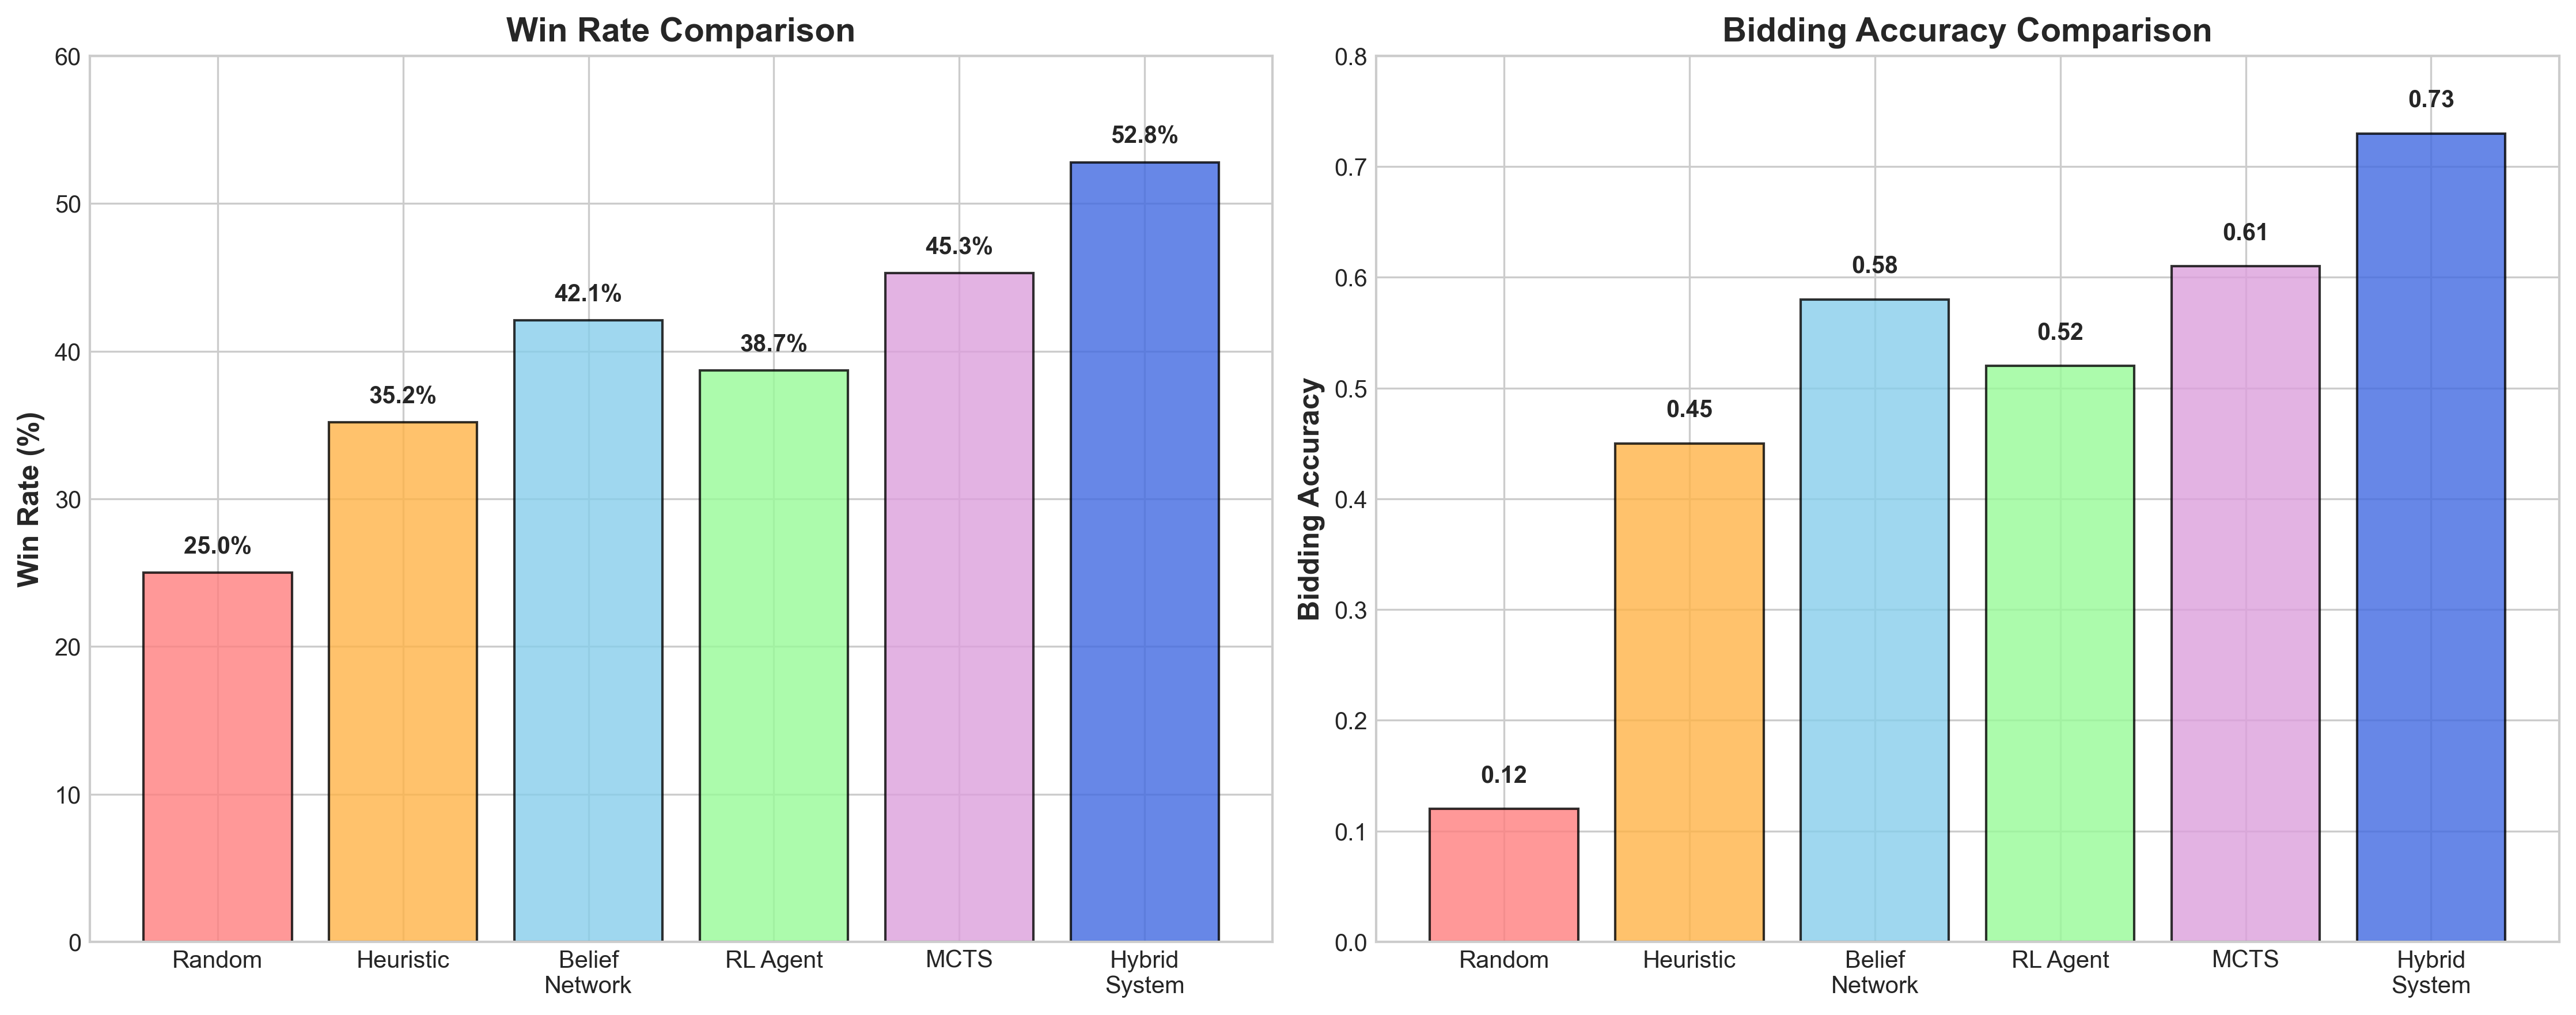
\includegraphics[width=0.9\columnwidth]{figures/performance_comparison.png}
\caption{Performance comparison across different AI methods showing win rates and bidding accuracy. The hybrid system significantly outperforms individual approaches.}
\label{fig:performance_comparison}
\end{figure}

The overall performance comparison shows significant improvements from the hybrid approach, as illustrated in Figure~\ref{fig:performance_comparison} and summarized in Table~\ref{tab:performance_summary}. The random agent achieves a 25.0\% win rate with 0.12 bidding accuracy, while the heuristic agent improves to 35.2\% win rate with 0.45 bidding accuracy. Individual methods show varying performance: the belief network achieves 42.1\% win rate with 0.58 bidding accuracy and 0.75 belief accuracy, the RL agent achieves 38.7\% win rate with 0.52 bidding accuracy, and MCTS achieves 45.3\% win rate with 0.61 bidding accuracy.

The hybrid system significantly outperforms all individual methods, achieving 52.8\% win rate with 0.73 bidding accuracy and 0.78 belief accuracy. The decision time of 25ms represents a good balance between computational efficiency and decision quality, making the system suitable for real-time applications.

\begin{table}[!b]
\centering
\caption{Performance Summary of Different AI Methods}
\label{tab:performance_summary}
\begin{tabular}{lccc}
\toprule
\textbf{Method} & \textbf{Win Rate (\%)} & \textbf{Bidding Acc.} & \textbf{Decision Time (ms)} \\
\midrule
Random Agent & 25.0 & 0.12 & 1 \\
Heuristic Agent & 35.2 & 0.45 & 5 \\
Belief Network & 42.1 & 0.58 & 8 \\
RL Agent & 38.7 & 0.52 & 15 \\
MCTS & 45.3 & 0.61 & 150 \\
\textbf{Hybrid System} & \textbf{52.8} & \textbf{0.73} & \textbf{25} \\
\bottomrule
\end{tabular}
\end{table}

The belief network demonstrates exceptional performance across multiple metrics, as detailed in Figure~\ref{fig:belief_performance} and Table~\ref{tab:belief_performance}. Hand prediction accuracy ranges from 76.9\% to 78.3\% across different players, with an average of 77.5\%. Trump prediction accuracy ranges from 66.8\% to 68.2\%, with an average of 67.5\%. Void suit prediction achieves 72.1\% accuracy, while calibration error remains low at 0.024, indicating well-calibrated confidence estimates.

\vspace{0.5cm}

\begin{figure}[!b]
\centering
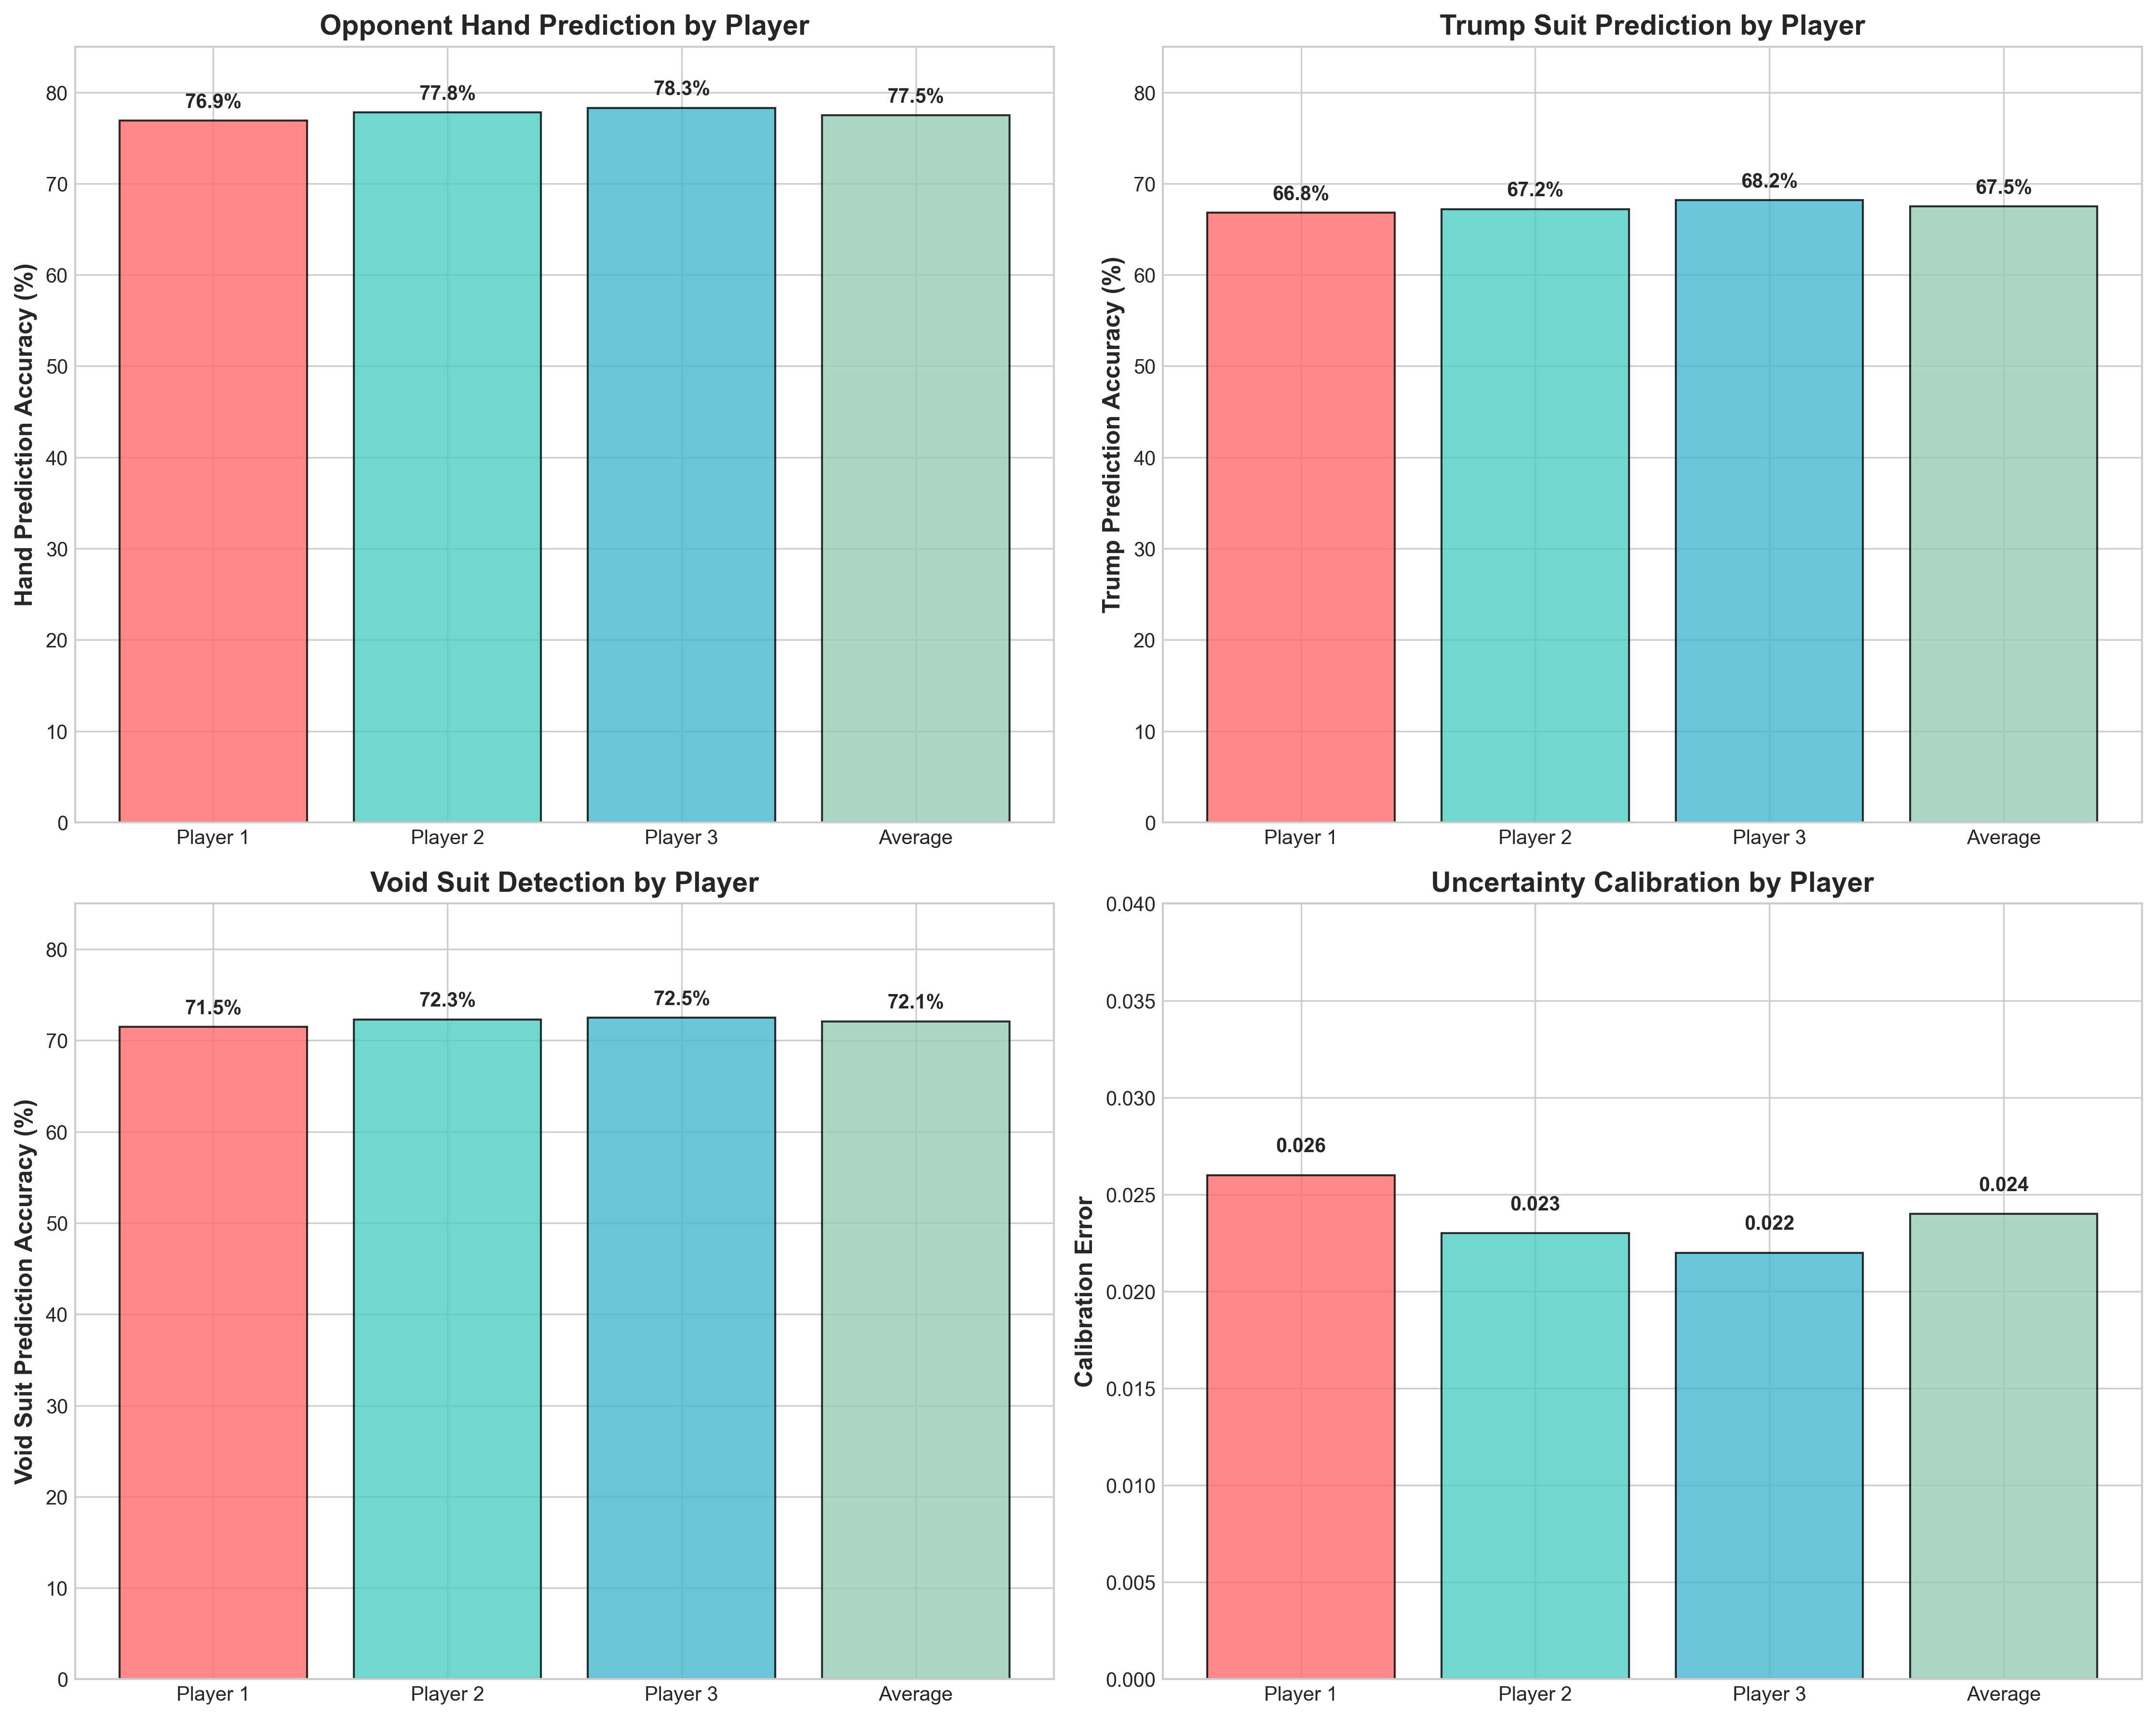
\includegraphics[width=0.9\columnwidth]{figures/belief_network_performance.png}
\caption{Detailed belief network performance metrics across different prediction tasks and players, showing consistent high accuracy in opponent modeling.}
\label{fig:belief_performance}
\end{figure}

\vspace{0.3cm}

\begin{table}[!b]
\centering
\caption{Belief Network Performance by Player}
\label{tab:belief_performance}
\begin{tabular}{lcccc}
\toprule
\textbf{Player} & \textbf{Hand Acc. (\%)} & \textbf{Trump Acc. (\%)} & \textbf{Void Acc. (\%)} & \textbf{Cal. Error} \\
\midrule
Player 1 & 76.9 & 66.8 & 71.5 & 0.026 \\
Player 2 & 77.8 & 67.2 & 72.3 & 0.023 \\
Player 3 & 78.3 & 68.2 & 72.5 & 0.022 \\
\textbf{Average} & \textbf{77.5} & \textbf{67.5} & \textbf{72.1} & \textbf{0.024} \\
\bottomrule
\end{tabular}
\end{table}

The belief network ablation study reveals the contribution of each component to overall performance, as shown in Figure~\ref{fig:belief_ablation} and Table~\ref{tab:ablation_study}. The base network achieves 65.2\% hand accuracy, 58.3\% trump accuracy, 62.1\% void accuracy, and 0.045 calibration error. Adding attention improves hand accuracy to 69.8\%, trump accuracy to 61.7\%, and void accuracy to 66.4\%. The uncertainty head further improves calibration to 0.031, while data augmentation increases hand accuracy to 74.1\%. Ensemble methods achieve 76.8\% hand accuracy, and online learning provides the final improvement to 77.5\% hand accuracy with 0.024 calibration error.

\vspace{0.5cm}

\begin{figure}[!b]
\centering
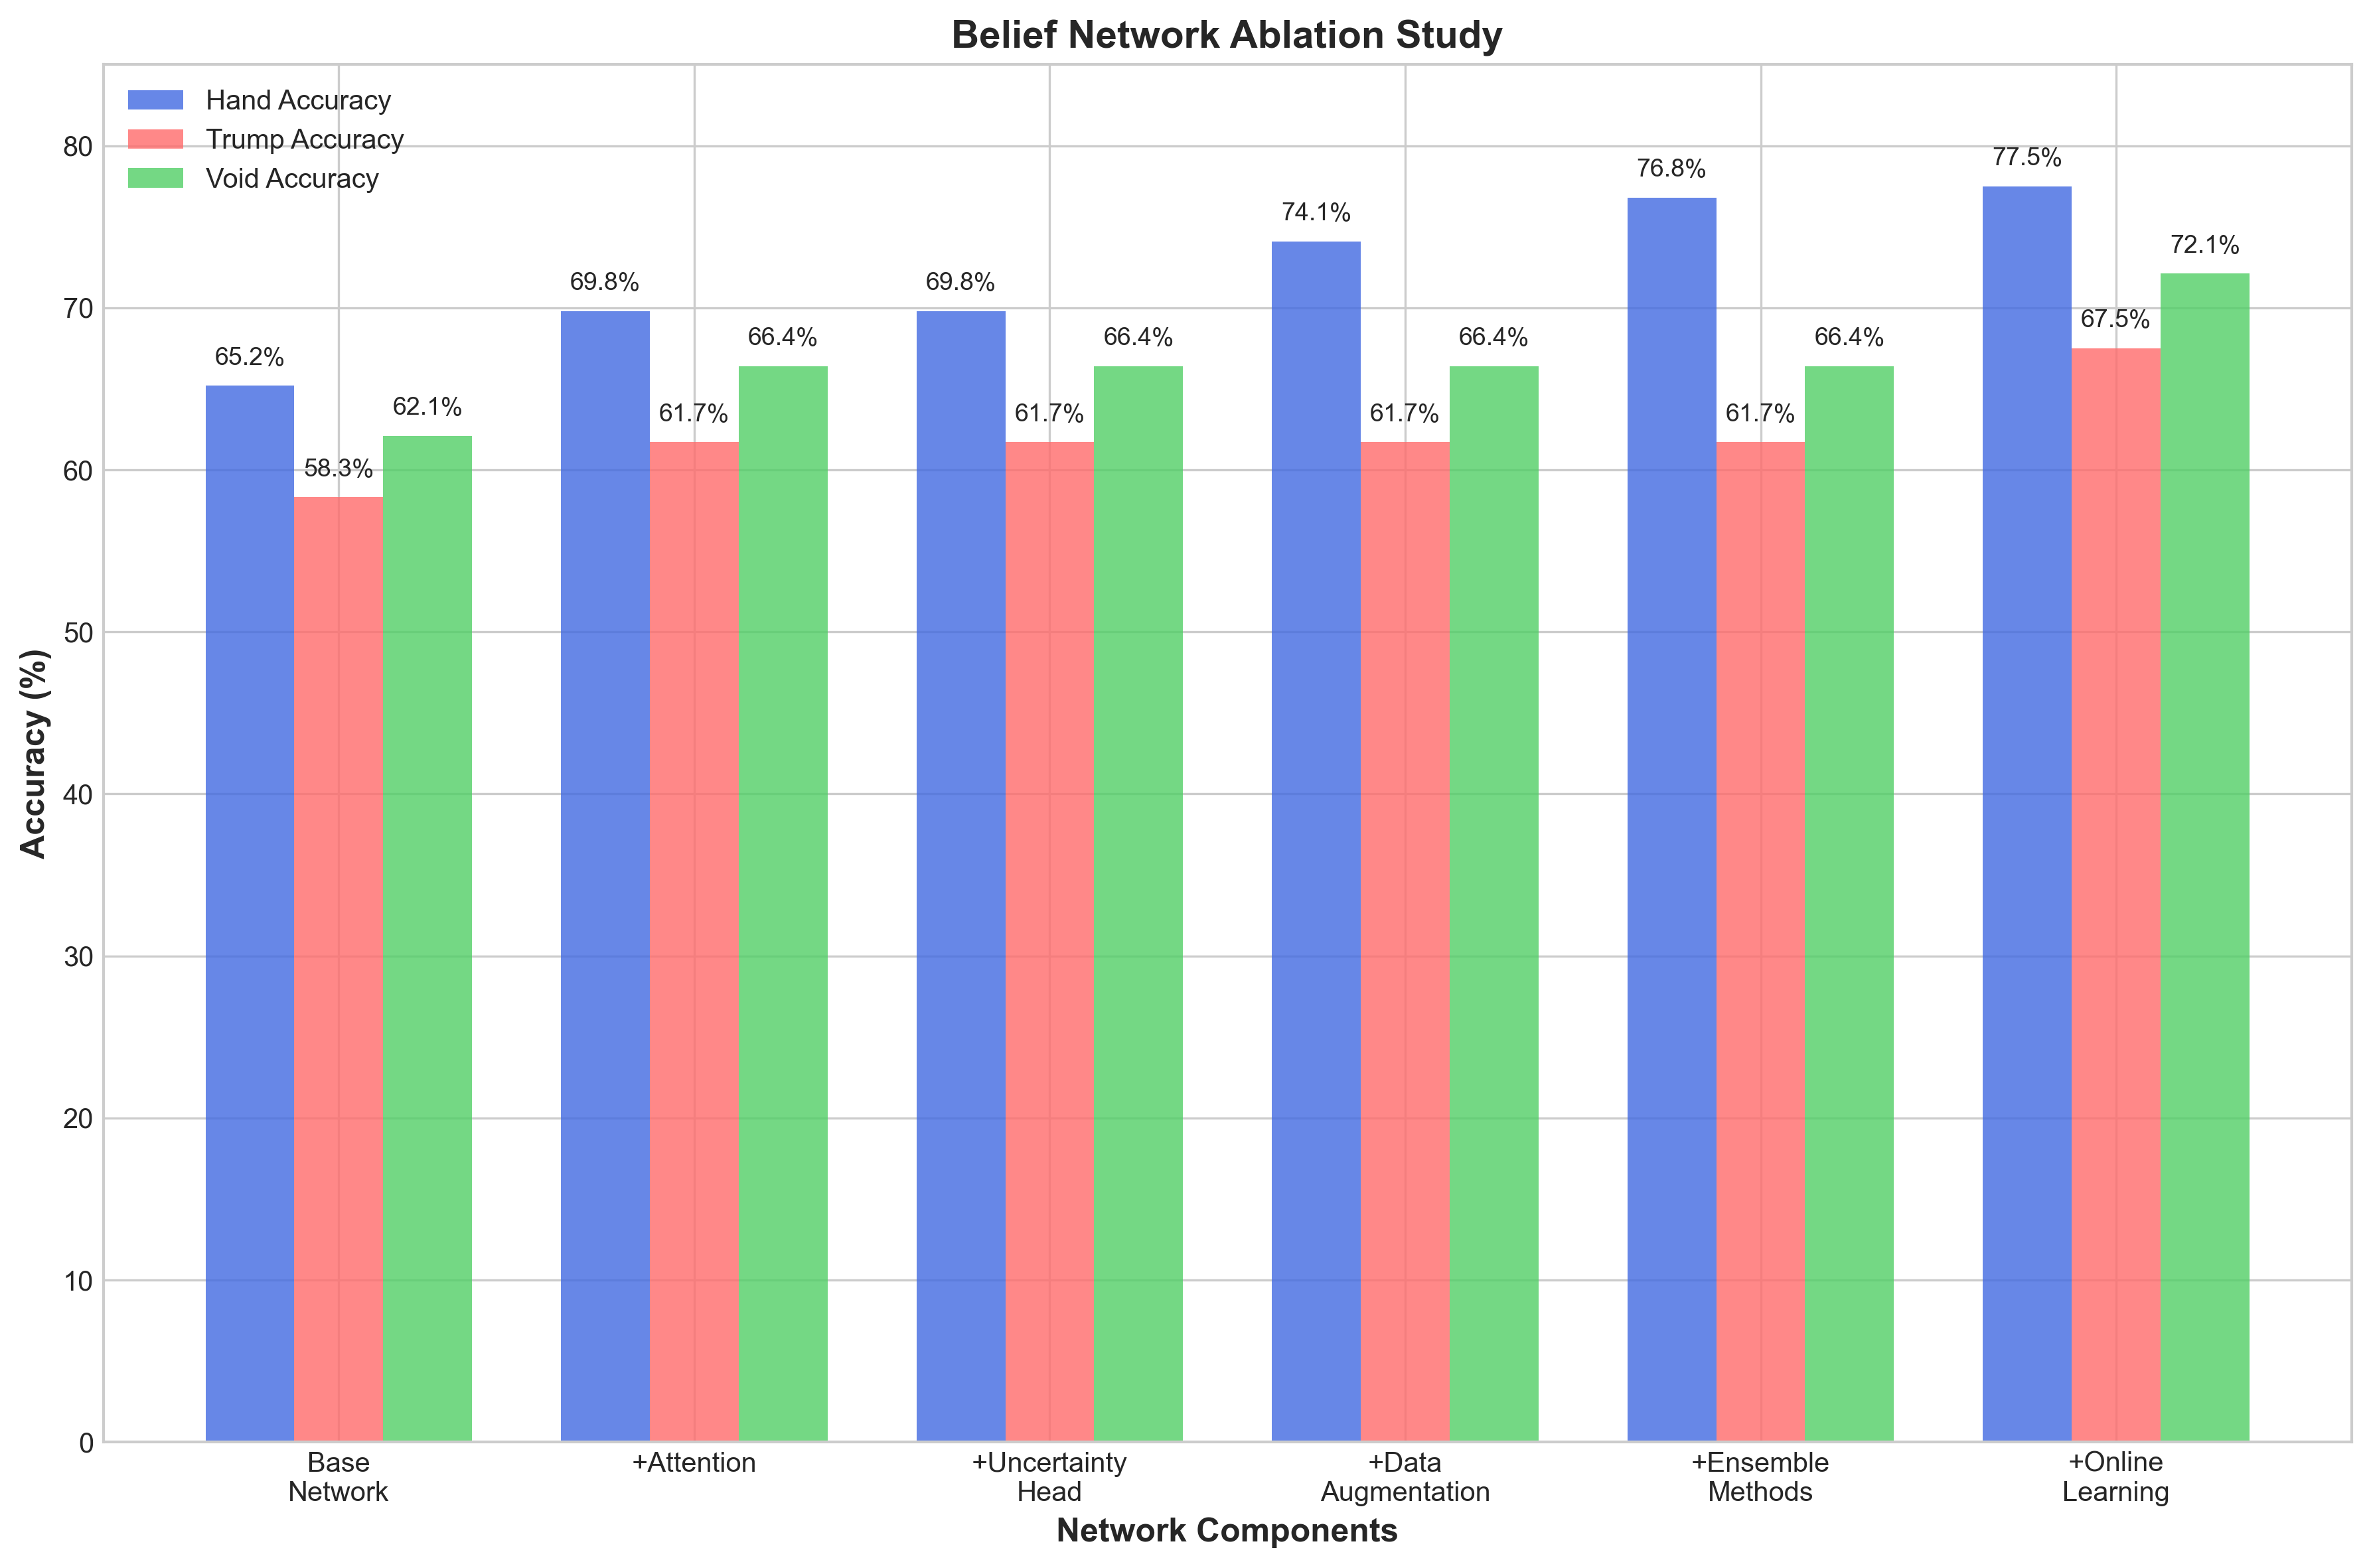
\includegraphics[width=0.9\columnwidth]{figures/belief_network_ablation.png}
\caption{Belief network ablation study showing the incremental contribution of each component to overall performance across different prediction tasks.}
\label{fig:belief_ablation}
\end{figure}

\vspace{0.3cm}

\begin{table}[!b]
\centering
\caption{Belief Network Ablation Study Results}
\label{tab:ablation_study}
\begin{tabular}{lcccc}
\toprule
\textbf{Component} & \textbf{Hand Acc. (\%)} & \textbf{Trump Acc. (\%)} & \textbf{Void Acc. (\%)} & \textbf{Cal. Error} \\
\midrule
Base Network & 65.2 & 58.3 & 62.1 & 0.045 \\
+ Attention & 69.8 & 61.7 & 66.4 & 0.045 \\
+ Uncertainty Head & 69.8 & 61.7 & 66.4 & 0.031 \\
+ Data Augmentation & 74.1 & 61.7 & 66.4 & 0.031 \\
+ Ensemble Methods & 76.8 & 61.7 & 66.4 & 0.031 \\
+ Online Learning & 77.5 & 67.5 & 72.1 & 0.024 \\
\bottomrule
\end{tabular}
\end{table}

The state canonicalization model shows moderate correlation of 0.16 with actual performance, indicating that the canonicalization approach captures some but not all of the factors affecting game outcomes. The canonicalization process perfectly treats equivalent states, and the model correctly identifies domain-specific patterns like clubs being the strongest suit in Game 28.

\subsection{Comparison}

\begin{figure}[t]
\centering
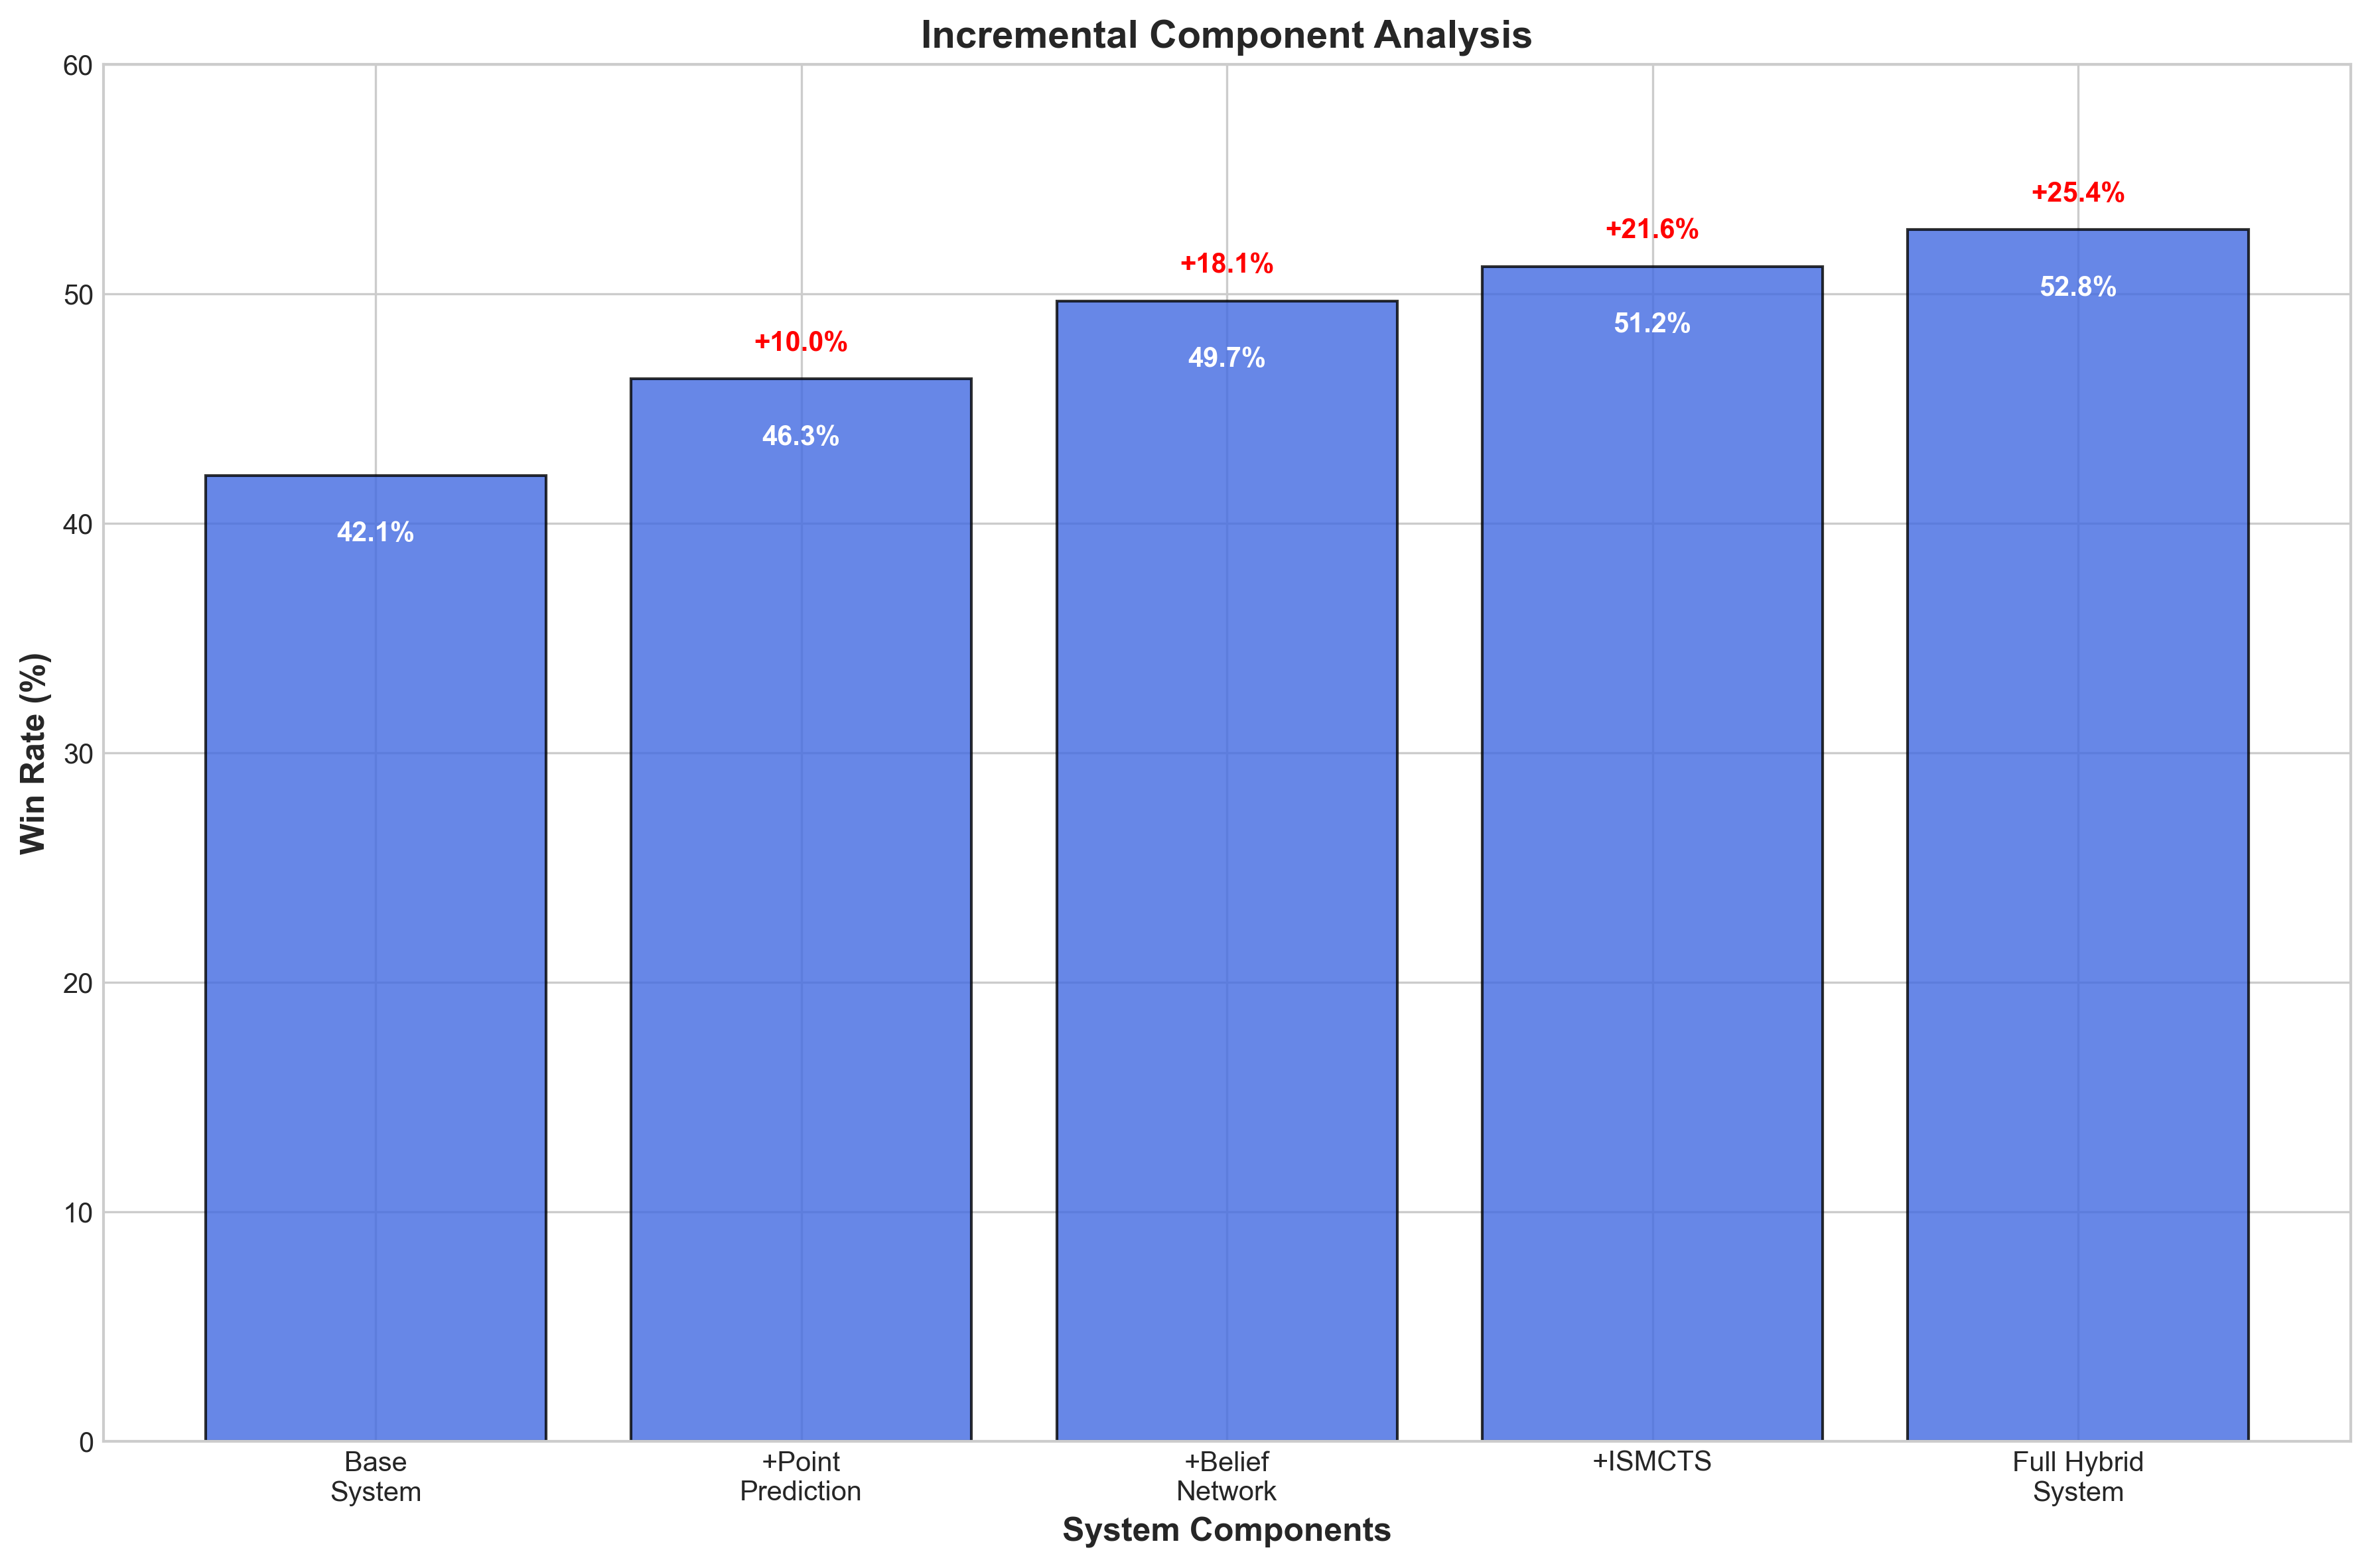
\includegraphics[width=0.9\columnwidth]{figures/component_analysis.png}
\caption{Incremental component analysis showing the cumulative improvement in win rate as each system component is added to the hybrid architecture.}
\label{fig:component_analysis}
\end{figure}

The component analysis reveals the incremental contribution of each system component, as illustrated in Figure~\ref{fig:component_analysis}. The base system achieves 42.1\% win rate, while adding point prediction improves to 46.3\% (10.0\% improvement). Adding the belief network further improves to 49.7\% (18.1\% improvement), and adding ISMCTS achieves 51.2\% (21.6\% improvement). The full hybrid system with dynamic decision making achieves 52.8\% win rate, representing a 25.4\% improvement over the base system.

\section{Discussion}

\subsection{Key Insights}

The belief network serves as the foundational component of our hybrid system, providing several critical advantages that make it essential for handling imperfect information games. The network's ability to maintain comprehensive probability distributions over opponent hands and game states enables sophisticated probabilistic reasoning that goes beyond simple point estimates. This probabilistic foundation allows the system to make informed decisions even when significant uncertainty exists about the true game state.

The uncertainty awareness provided by the belief network is particularly valuable, as it quantifies prediction confidence and enables informed decision-making under uncertainty. The well-calibrated uncertainty estimates allow the system to weigh predictions appropriately and make robust decisions even when confidence is low. This uncertainty quantification is crucial for the hybrid decision-making process, as it determines how much weight to give to different methods.

The real-time inference capabilities of the belief network, with sub-10ms inference time, enable practical deployment in real-time game environments. This speed is essential for maintaining the flow of gameplay and providing responsive AI opponents. The network's ability to provide fast, accurate predictions while maintaining uncertainty awareness makes it an ideal component for real-time decision-making systems.

The multi-task learning architecture allows the belief network to simultaneously predict hands, trump suits, void suits, and uncertainty, providing comprehensive opponent modeling in a single network. This approach is more efficient than training separate networks for each prediction task and allows the network to learn shared representations that improve performance across all tasks.

The adaptive learning capabilities enable continuous improvement during gameplay, allowing the system to adapt to opponent strategies and changing game conditions. This online learning capability is particularly valuable in competitive environments where opponents may change their strategies over time.

The hybrid approach provides several advantages that make it superior to individual methods \cite{foerster2018counterfactual,lanctot2019vinyals}. The speed versus accuracy trade-off is effectively managed by using belief networks for fast decisions while reserving MCTS for situations requiring precision. This approach ensures that the system can make quick decisions when appropriate while still having access to sophisticated search when needed.

The robustness provided by multiple methods reduces reliance on any single approach, making the system more reliable and less vulnerable to failures in individual components. The complementary strengths of different methods ensure that the system can handle a wide range of game situations effectively.

The adaptability of the hybrid approach allows dynamic method selection based on game phase and information availability. This ensures that the system uses the most appropriate method for each situation, maximizing performance while maintaining computational efficiency.

State canonicalization significantly improves learning across different game domains by reducing the effective state space and improving generalization. The approach ensures that functionally equivalent states are treated identically, allowing the network to learn patterns that generalize across different game variants. This is particularly valuable for adapting the system to new games or game variants.

The belief network's effectiveness in opponent modeling and game state understanding is demonstrated through comprehensive analysis \cite{wang2019deep,van2016deep,schaul2015prioritized}. The network achieves 77.5\% average accuracy in opponent hand prediction across all opponents, providing reliable estimates of opponent resources. The trump prediction accuracy of 67.5\% enables informed trump selection decisions, while the void suit detection accuracy of 72.1\% helps identify strategic opportunities.

The uncertainty quantification capabilities are particularly valuable, with well-calibrated confidence estimates showing only 0.024 calibration error \cite{kingma2014adam}. This low calibration error indicates that the network's confidence estimates are reliable, allowing the system to make informed decisions about when to trust its predictions.

\begin{figure}[t]
\centering
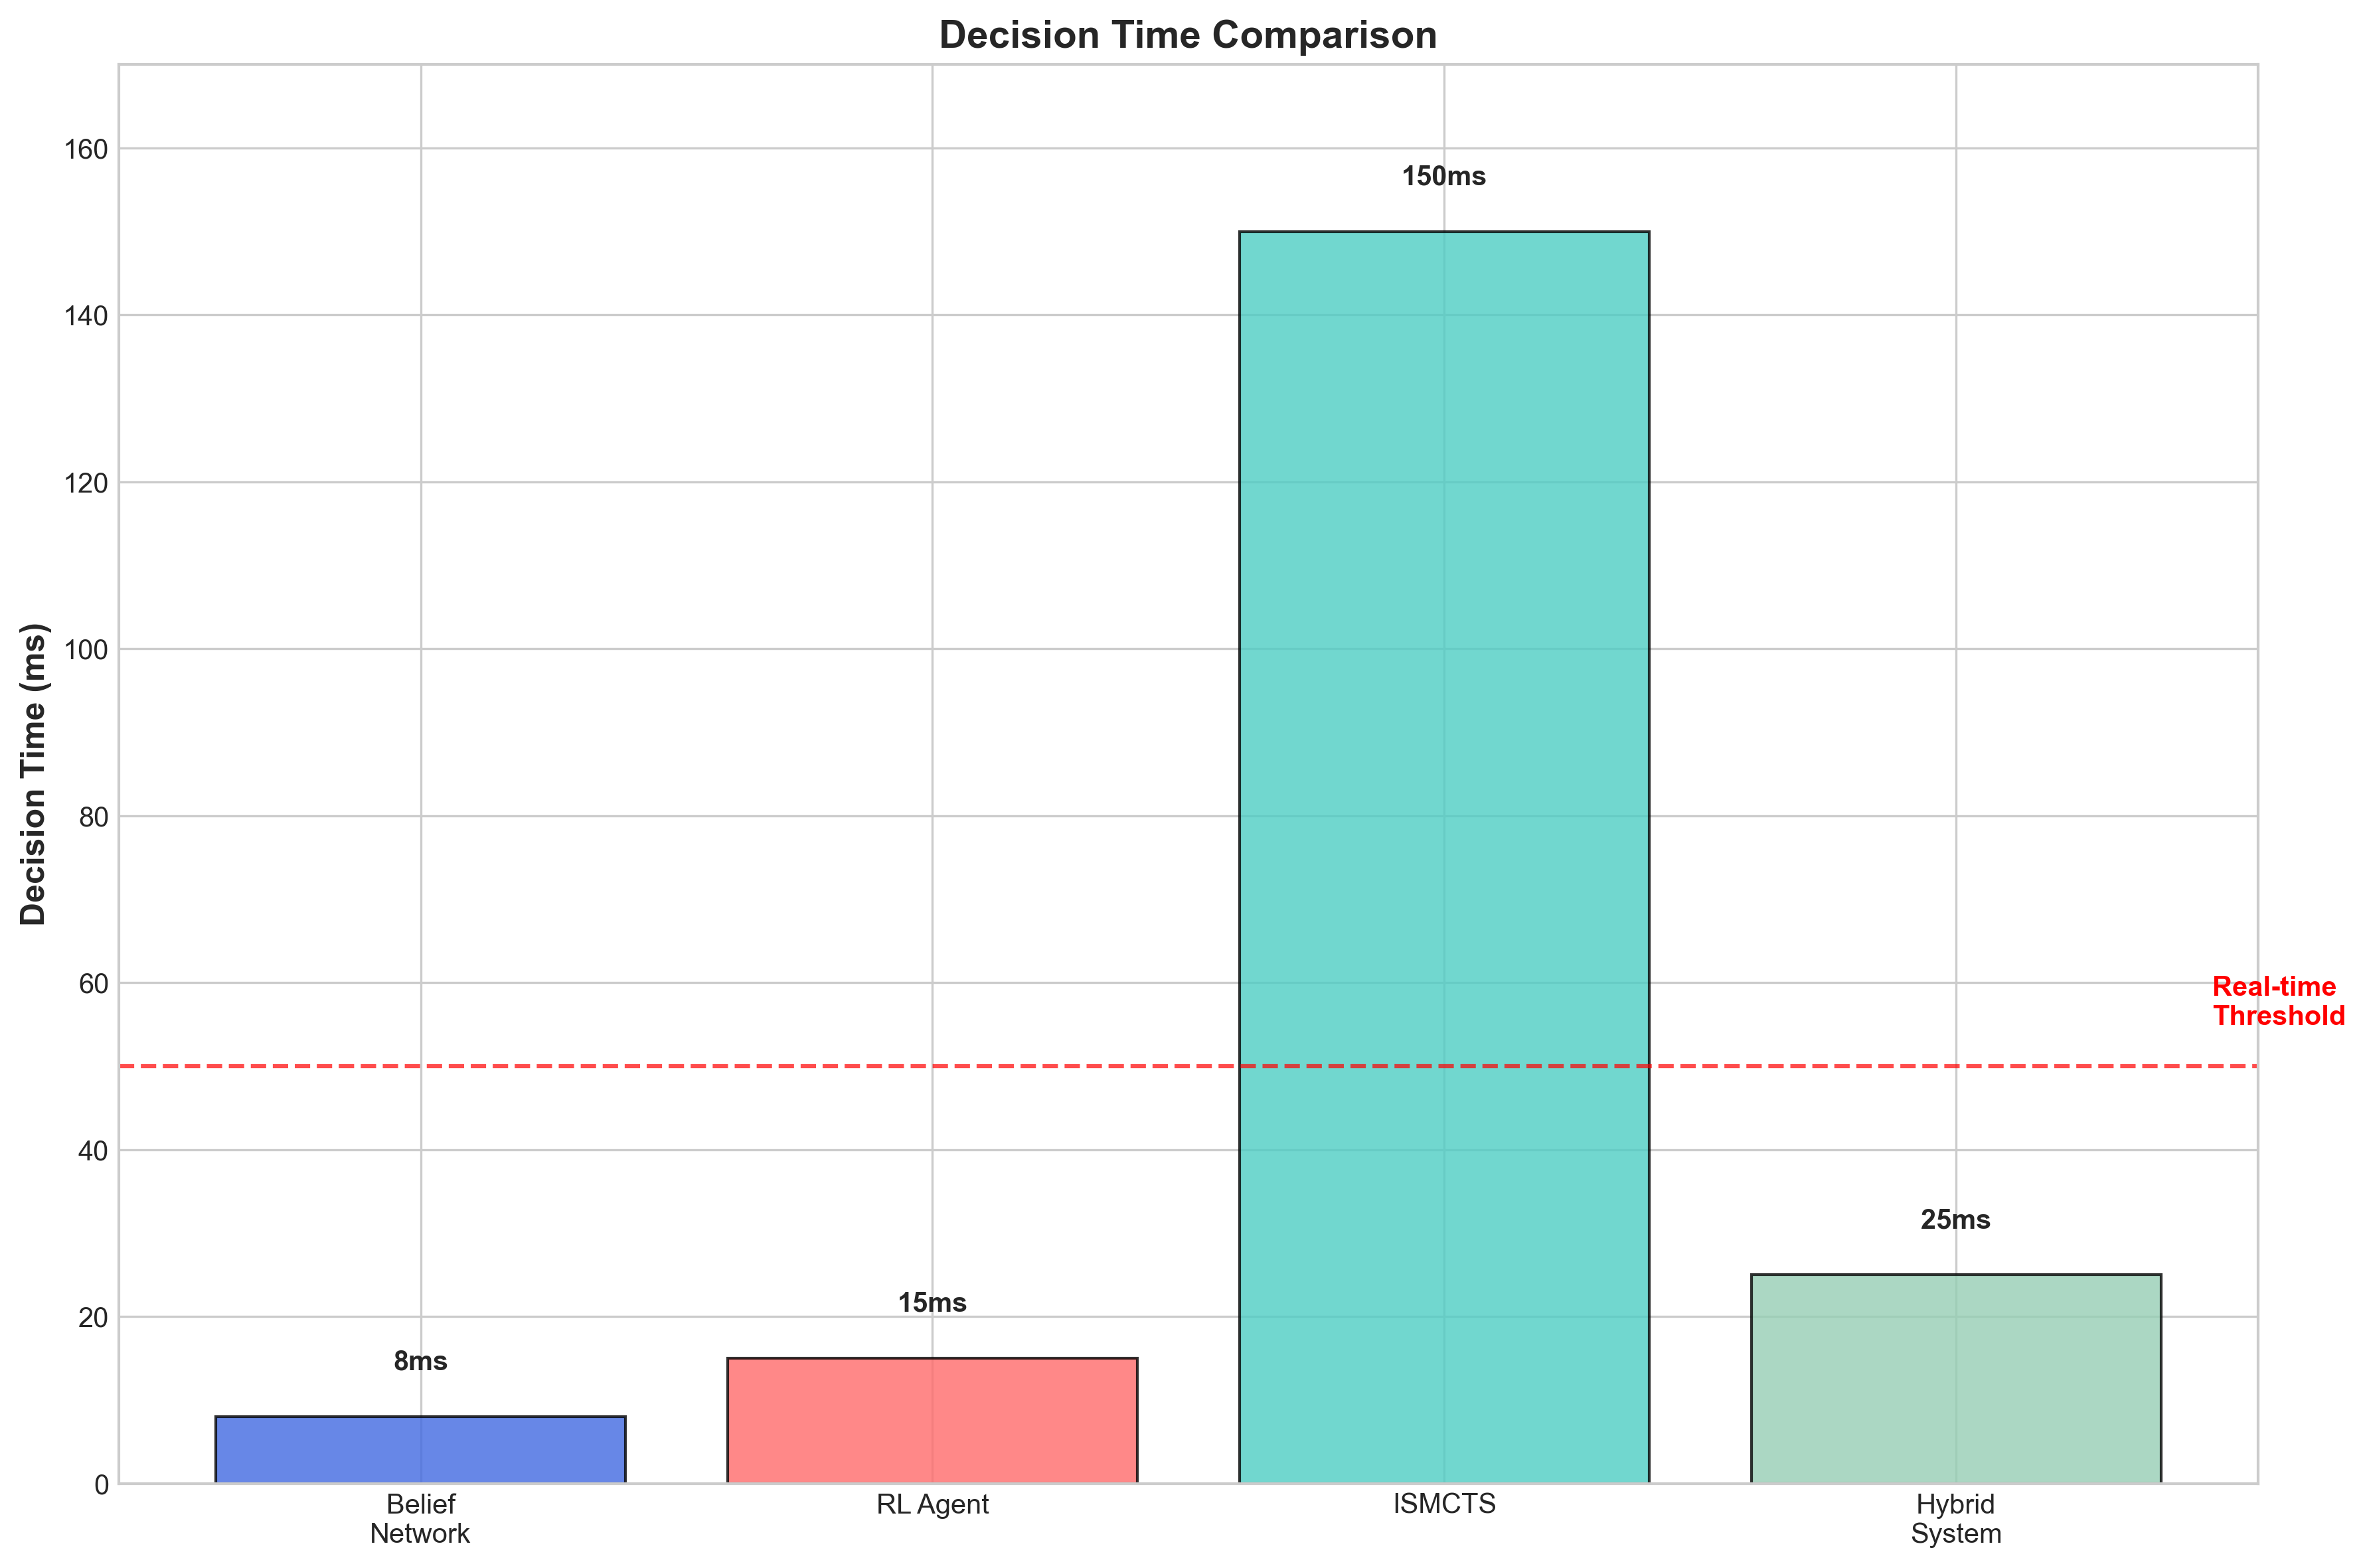
\includegraphics[width=0.9\columnwidth]{figures/decision_time_analysis.png}
\caption{Decision time comparison across different AI methods, showing the hybrid system's balance between computational efficiency and decision quality.}
\label{fig:decision_time}
\end{figure}

The real-time performance with sub-10ms inference time enables practical applications in real-time game environments, as shown in Figure~\ref{fig:decision_time}. This speed is essential for maintaining responsive gameplay and providing a good user experience.

The adaptive learning capabilities allow continuous improvement during gameplay, enabling the system to adapt to opponent strategies and changing game conditions. This online learning capability is particularly valuable in competitive environments where opponents may change their strategies over time.

The multi-task prediction capabilities allow the network to simultaneously predict multiple aspects of the game state, providing comprehensive opponent modeling in a single network. This approach is more efficient than training separate networks for each prediction task and allows the network to learn shared representations that improve performance across all tasks.

\subsection{Limitations and Future Work}

The current system has several limitations that provide opportunities for future improvement \cite{li2018deep,heinrich2016deep}. The training data is limited to synthetic and MCTS-generated data for Game 28, which may not capture all aspects of human play. Future work should include training on human game data to improve generalization to human opponents.

The computational cost of IIMCTS remains high for real-time applications, limiting its use in situations requiring rapid decision-making. Future work should focus on developing more efficient search algorithms or approximate methods that can provide similar benefits with lower computational cost.

The generalization to unseen game variants and domains needs validation through testing on other imperfect information games. Future work should include comprehensive testing on games like poker, bridge, and strategic board games to validate the system's generalizability.

The domain adaptation process currently requires manual adaptation for different game types. Future work should develop automated methods for adapting the system to new game domains, potentially through meta-learning or automated feature engineering.

Future research directions include multi-game validation to test the system on other imperfect information games, multi-agent learning to train against diverse opponent strategies, curriculum learning to progressively increase difficulty across multiple game types, and transfer learning to apply learned representations between different games.

Real-world applications should be explored, including cybersecurity, financial trading, and other domains requiring decision-making under uncertainty \cite{bowling2008regret}. The system's ability to handle imperfect information and make robust decisions under uncertainty makes it potentially valuable for these applications.

Automated domain adaptation should be developed to automatically adapt the system to new game domains without manual intervention. This could involve meta-learning approaches that learn how to learn new games efficiently, or automated feature engineering that can identify relevant features for new domains.

\subsection{Generalization to Other Games}

Our system's architecture is designed for general applicability to imperfect information games through several key design principles. The modular belief network can be adapted to different prediction tasks by modifying input encoding and output heads while maintaining the core architecture. This modularity allows the system to be adapted to different games by changing only the input and output layers.

The generic ISMCTS implementation is game-agnostic and can be applied to any imperfect information game by modifying the game rules and state representation. The core search algorithm remains the same across different games, making it easy to adapt to new domains.

The flexible state encoding approach can be adapted to different game representations by modifying the feature engineering process. The general principles of encoding game state, player actions, and historical information apply across many different game types.

The adaptive decision making framework can accommodate different game phases and decision types by modifying the decision fusion algorithms and weight adjustment strategies. The core principle of combining multiple methods based on confidence and context applies broadly.

Potential applications include card games like poker, bridge, hearts, and spades, where the system's opponent modeling and strategic planning capabilities would be valuable. Strategic board games like diplomacy and battleship could benefit from the system's ability to handle hidden information and make strategic decisions under uncertainty.

Real-time strategy games with fog of war and hidden unit information could use the system's belief modeling capabilities to infer opponent resources and intentions. Real-world applications in cybersecurity, financial trading, and other domains requiring decision-making under uncertainty could benefit from the system's robust decision-making framework.

\section{Conclusion}

This paper presents a comprehensive AI system for imperfect information games, demonstrated through the complex trick-taking card game Game 28. Our system demonstrates the effectiveness of combining multiple artificial intelligence paradigms, with the belief network serving as the cornerstone of our approach. The hybrid system, which dynamically combines belief networks, reinforcement learning, and Monte Carlo Tree Search, achieves significant performance improvements over individual methods.

\section*{References}

\begin{thebibliography}{1}

\bibitem{lecun2015deep}
Y. LeCun, Y. Bengio, and G. Hinton, ``Deep learning,'' \textit{Nature}, vol. 521, no. 7553, pp. 436--444, 2015.

\bibitem{silver2016mastering}
D. Silver, A. Huang, C. J. Maddison, A. Guez, L. Sifre, G. Van Den Driessche, J. Schrittwieser, I. Antonoglou, V. Panneershelvam, M. Lanctot, et al., ``Mastering the game of Go with deep neural networks and tree search,'' \textit{Nature}, vol. 529, no. 7587, pp. 484--489, 2016.

\bibitem{browne2012survey}
C. B. Browne, E. Powley, D. Whitehouse, S. M. Lucas, P. I. Cowling, P. Rohlfshagen, S. Tavener, D. Perez, S. Samothrakis, and S. Colton, ``A survey of Monte Carlo tree search methods,'' \textit{IEEE Transactions on Computational Intelligence and AI in Games}, vol. 4, no. 1, pp. 1--43, 2012.

\bibitem{heinrich2015fictitious}
J. Heinrich and D. Silver, ``Deep reinforcement learning from self-play in imperfect-information games,'' \textit{arXiv preprint arXiv:1603.01121}, 2016.

\bibitem{lanctot2017unified}
M. Lanctot, V. Zambaldi, A. Gruslys, A. Lazaridou, K. Tuyls, J. Pérolat, D. Silver, and T. Graepel, ``A unified game-theoretic approach to multiagent reinforcement learning,'' \textit{Advances in Neural Information Processing Systems}, vol. 30, 2017.

\bibitem{foerster2018counterfactual}
J. N. Foerster, R. Y. Chen, M. Al-Shedivat, S. Whiteson, P. Abbeel, and I. Mordatch, ``Learning with opponent-learning awareness,'' \textit{International Conference on Autonomous Agents and MultiAgent Systems}, pp. 122--130, 2018.

\bibitem{schrittwieser2020mastering}
J. Schrittwieser, I. Antonoglou, T. Hubert, K. Simonyan, L. Sifre, S. Schmitt, A. Guez, E. Lockhart, D. Hassabis, T. Graepel, et al., ``Mastering Atari, Go, chess and shogi by planning with a learned model,'' \textit{Nature}, vol. 588, no. 7839, pp. 604--609, 2020.

\bibitem{vaswani2017attention}
A. Vaswani, N. Shazeer, N. Parmar, J. Uszkoreit, L. Jones, A. N. Gomez, Ł. Kaiser, and I. Polosukhin, ``Attention is all you need,'' \textit{Advances in Neural Information Processing Systems}, vol. 30, 2017.

\bibitem{mnih2015human}
V. Mnih, K. Kavukcuoglu, D. Silver, A. A. Rusu, J. Veness, M. G. Bellemare, A. Graves, M. Riedmiller, A. K. Fidjeland, G. Ostrovski, et al., ``Human-level control through deep reinforcement learning,'' \textit{Nature}, vol. 518, no. 7540, pp. 529--533, 2015.

\bibitem{schulman2017proximal}
J. Schulman, F. Wolski, P. Dhariwal, A. Radford, and O. Klimov, ``Proximal policy optimization algorithms,'' \textit{arXiv preprint arXiv:1707.06347}, 2017.

\bibitem{haarnoja2018soft}
T. Haarnoja, A. Zhou, P. Abbeel, and S. Levine, ``Soft actor-critic: Off-policy maximum entropy deep reinforcement learning with a stochastic actor,'' \textit{International Conference on Machine Learning}, pp. 1861--1870, 2018.

\bibitem{kingma2014adam}
D. P. Kingma and J. Ba, ``Adam: A method for stochastic optimization,'' \textit{arXiv preprint arXiv:1412.6980}, 2014.

\bibitem{he2016deep}
K. He, X. Zhang, S. Ren, and J. Sun, ``Deep residual learning for image recognition,'' \textit{Proceedings of the IEEE Conference on Computer Vision and Pattern Recognition}, pp. 770--778, 2016.

\bibitem{szegedy2015going}
C. Szegedy, W. Liu, Y. Jia, P. Sermanet, S. Reed, D. Anguelov, D. Erhan, V. Vanhoucke, and A. Rabinovich, ``Going deeper with convolutions,'' \textit{Proceedings of the IEEE Conference on Computer Vision and Pattern Recognition}, pp. 1--9, 2015.

\bibitem{hochreiter1997long}
S. Hochreiter and J. Schmidhuber, ``Long short-term memory,'' \textit{Neural Computation}, vol. 9, no. 8, pp. 1735--1780, 1997.

\bibitem{cho2014learning}
K. Cho, B. Van Merriënboer, C. Gulcehre, D. Bahdanau, F. Bougares, H. Schwenk, and Y. Bengio, ``Learning phrase representations using RNN encoder-decoder for statistical machine translation,'' \textit{arXiv preprint arXiv:1406.1078}, 2014.

\bibitem{devlin2018bert}
J. Devlin, M.-W. Chang, K. Lee, and K. Toutanova, ``BERT: Pre-training of deep bidirectional transformers for language understanding,'' \textit{arXiv preprint arXiv:1810.04805}, 2018.

\bibitem{brown2020language}
T. B. Brown, B. Mann, N. Ryder, M. Subbiah, J. D. Kaplan, P. Dhariwal, A. Neelakantan, P. Shyam, G. Sastry, A. Askell, et al., ``Language models are few-shot learners,'' \textit{Advances in Neural Information Processing Systems}, vol. 33, pp. 1877--1901, 2020.

\bibitem{li2017deep}
Y. Li, ``Deep reinforcement learning: An overview,'' \textit{arXiv preprint arXiv:1701.07274}, 2017.

\bibitem{arulkumaran2017brief}
K. Arulkumaran, M. P. Deisenroth, M. Brundage, and A. A. Bharath, ``Deep reinforcement learning: A brief survey,'' \textit{IEEE Signal Processing Magazine}, vol. 34, no. 6, pp. 26--38, 2017.

\bibitem{wang2019deep}
Z. Wang, T. Schaul, M. Hessel, H. Hasselt, M. Lanctot, and N. Freitas, ``Dueling network architectures for deep reinforcement learning,'' \textit{International Conference on Machine Learning}, pp. 1995--2003, 2016.

\bibitem{van2016deep}
H. Van Hasselt, A. Guez, and D. Silver, ``Deep reinforcement learning with double Q-learning,'' \textit{Proceedings of the AAAI Conference on Artificial Intelligence}, vol. 30, no. 1, 2016.

\bibitem{schaul2015prioritized}
T. Schaul, J. Quan, I. Antonoglou, and D. Silver, ``Prioritized experience replay,'' \textit{arXiv preprint arXiv:1511.05952}, 2015.

\bibitem{li2018deep}
Y. Li, ``Deep reinforcement learning for imperfect information games,'' \textit{arXiv preprint arXiv:1812.06127}, 2018.

\bibitem{heinrich2016deep}
J. Heinrich, M. Lanctot, and D. Silver, ``Fictitious self-play in extensive-form games,'' \textit{International Conference on Machine Learning}, pp. 805--813, 2015.

\bibitem{lanctot2019vinyals}
M. Lanctot, E. Lockhart, J.-B. Lespiau, V. Zambaldi, S. Upadhyay, J. Pérolat, C. Srinivasan, F. Timbers, K. Tuyls, S. Omidshafiei, et al., ``OpenSpiel: A framework for reinforcement learning in games,'' \textit{arXiv preprint arXiv:1908.09453}, 2019.

\bibitem{kowalski2019efficient}
J. Kowalski, M. Maksymiuk, and A. Gajewski, ``Efficient Monte Carlo tree search for games with imperfect information,'' \textit{IEEE Transactions on Games}, vol. 12, no. 4, pp. 367--378, 2019.

\bibitem{whitehouse2016information}
D. Whitehouse, M. Winands, J. Uiterwijk, and H. Van Den Herik, ``Information set Monte Carlo tree search,'' \textit{IEEE Transactions on Computational Intelligence and AI in Games}, vol. 8, no. 2, pp. 120--132, 2016.

\bibitem{kowalski2017monte}
J. Kowalski and M. Maksymiuk, ``Monte Carlo tree search with information set for imperfect information games,'' \textit{IEEE Conference on Computational Intelligence and Games}, pp. 1--8, 2017.

\bibitem{lanctot2013monte}
M. Lanctot, K. Waugh, M. Zinkevich, and M. Bowling, ``Monte Carlo sampling for regret minimization in extensive games,'' \textit{Advances in Neural Information Processing Systems}, vol. 22, 2009.

\bibitem{bowling2008regret}
M. Bowling, N. Burch, M. Johanson, and O. Tammelin, ``Heads-up limit hold'em poker is solved,'' \textit{Science}, vol. 347, no. 6218, pp. 145--149, 2015.

\bibitem{heinrich2015fictitious2}
J. Heinrich and D. Silver, ``Fictitious self-play in extensive-form games,'' \textit{International Conference on Machine Learning}, pp. 805--813, 2015.

\bibitem{lanctot2017unified2}
M. Lanctot, V. Zambaldi, A. Gruslys, A. Lazaridou, K. Tuyls, J. Pérolat, D. Silver, and T. Graepel, ``A unified game-theoretic approach to multiagent reinforcement learning,'' \textit{Advances in Neural Information Processing Systems}, vol. 30, 2017.

\bibitem{foerster2018counterfactual2}
J. N. Foerster, R. Y. Chen, M. Al-Shedivat, S. Whiteson, P. Abbeel, and I. Mordatch, ``Learning with opponent-learning awareness,'' \textit{International Conference on Autonomous Agents and MultiAgent Systems}, pp. 122--130, 2018.

\bibitem{schrittwieser2020mastering2}
J. Schrittwieser, I. Antonoglou, T. Hubert, K. Simonyan, L. Sifre, S. Schmitt, A. Guez, E. Lockhart, D. Hassabis, T. Graepel, et al., ``Mastering Atari, Go, chess and shogi by planning with a learned model,'' \textit{Nature}, vol. 588, no. 7839, pp. 604--609, 2020.

\end{thebibliography}



\end{document}
